\section{Optimización del rendimiento}

\begin{ejercicio}\label{ej:5.1}
    Un servidor dedicado a la reserva de billetes de una compañía de ferrocarriles tiene un tiempo medio de respuesta de 15 milisegundos por petición. Si por término medio hay 345 peticiones activas en el servidor, ¿cuál es su productividad? Exprese el resultado en peticiones por segundo.\\

    Sabemos que $R_0=\unit[15]{ms}$ y $N_0=345$ trabajos. Entonces, Por la Ley de Little la productividad del servidor es:
    \begin{equation*}
        X_0 = \dfrac{N_0}{R_0} = \dfrac{345}{15\cdot10^{-3}} = \unitfrac[23000]{peticiones}{s}
    \end{equation*}
        
\end{ejercicio}
\begin{comment}
\solucion
    La productividad del servidor es de 23000 peticiones por segundo.
\end{comment}

\begin{ejercicio}\label{ej:5.2}
    El servidor web de una compañía comercial ha servido 120 peticiones durante el último minuto. Si el número medio de peticiones activas ha sido de 5, calcule el tiempo medio de respuesta experimentado por una petición al servidor web.\\

    Tenemos que $C_0 = 120$ peticiones, $T = 60$ segundos y $N_0 = 5$ peticiones. En primer lugar, calculamos la productividad del servidor:
    \begin{equation*}
        X_0 = \dfrac{C_0}{T} = \dfrac{120}{60} = \unitfrac[2]{peticiones}{s}
    \end{equation*}

    Por tanto, el tiempo medio de respuesta del servidor es:
    \begin{equation*}
        R_0 = \dfrac{N_0}{X_0} = \dfrac{5}{2} = \unit[2.5]{s}
    \end{equation*}
\end{ejercicio}
\begin{comment}
\solucion
    El tiempo medio de respuesta es de 2,5 segundos.
\end{comment}

\begin{ejercicio}\label{ej:5.3}
    El computador de una empresa conservera se utiliza de manera interactiva por los 45 empleados que tiene en plantilla. Si el tiempo medio de reflexión es de 17 segundos y su productividad de $2.5$ peticiones por segundo, ¿cuál es el tiempo medio de respuesta de cada interacción?\\

    Sabemos que $Z = \unit[17]{s}$, $X_0 = \unitfrac[2.5]{peticiones}{s}$ y $N_0 = 45$ trabajos. Por la Ley del Tiempo de Respuesta Interactivo, el tiempo medio de respuesta del computador es:
    \begin{equation*}
        R_0 = \dfrac{N_0}{X_0} - Z  = \dfrac{45}{2.5} - 17 = \unit[18]{s} - \unit[17]{s} = \unit[1]{s}
    \end{equation*}
\end{ejercicio}
\begin{comment}
\solucion
    El tiempo medio de respuesta de cada interacción es de 1 segundo.
\end{comment}

\begin{ejercicio}\label{ej:5.4}
    Durante una sesión de medida de media hora un monitor software ha extraído las variables operacionales básicas de un disco duro mostradas en la Tabla~\ref{tab:5.4}.
    \begin{table}[h]
        \centering
        \begin{tabular}{|c|c|}
            \hline
            Variable & Valor \\
            \hline
            $A_i$ & 364 peticiones \\
            $C_i$ & 359 peticiones \\
            $B_i$ & 23 minutos \\
            \hline
        \end{tabular}
        \caption{Variables operacionales del disco duro.}
        \label{tab:5.4}
    \end{table}
    A partir de la información anterior calcule las siguientes variables operacionales deducidas del disco duro:
    \begin{enumerate}
        \item Tasa de llegada de peticiones al disco duro.
        
        Del enunciado, deducimos que $T = \unit[30]{min} = \unit[1800]{s}$. Por tanto, la tasa de llegada de peticiones al disco duro es:
        \begin{equation*}
            \lambda_i = \dfrac{A_i}{T} = \dfrac{364}{1800} = \unitfrac[0.2022]{peticiones}{s}
        \end{equation*}
        \item Productividad del disco duro.
        
        La productividad del disco duro es:
        \begin{equation*}
            X_i = \dfrac{C_i}{T} = \dfrac{359}{1800} = \unitfrac[0.1994]{peticiones}{s}
        \end{equation*}
        \item Utilización del disco duro.
        
        La utilización del disco duro es:
        \begin{equation*}
            U_i = \dfrac{B_i}{T} = \dfrac{23\cdot60}{1800} = \dfrac{23}{30} = 0.7667 = 76.67\%
        \end{equation*}
        \item Tiempo medio de servicio del disco duro.
        
        El tiempo medio de servicio del disco duro es:
        \begin{equation*}
            S_i = \dfrac{B_i}{C_i} = \dfrac{23\cdot60}{359} = \unitfrac[3.84]{s}{trabajo}
        \end{equation*}
    \end{enumerate}
\end{ejercicio}
\begin{comment}
\solucion
    \begin{itemize}
        \item $\lambda = 12.13$ peticiones/minuto
        \item $X = 11.97$ peticiones/minuto
        \item $U = 0.77$
        \item $S = 3.84$ segundos/petición
    \end{itemize}
\end{comment}

\begin{ejercicio}\label{ej:5.5}
    El sistema informático dedicado a la atención al cliente de una empresa de comestibles se puede modelar mediante una red de colas abierta con un procesador y dos unidades de disco. El comportamiento de cada petición se asemeja al modelo de servidor central. Se sabe que los tiempos de respuesta (expresados en milisegundos) y las razones de visita de estas estaciones son los mostrados en la Tabla~\ref{tab:5.5}.
    \begin{table}[h]
        \centering
        \begin{tabular}{|c|c|c|}
            \hline
            Estación & $V_i$ & $R_i$ \\
            \hline
            Procesador & 7 & 4.3 \\
            Disco 1 & 2 & 1.5 \\
            Disco 2 & 4 & 2.3 \\
            \hline
        \end{tabular}
        \caption{Tiempos de respuesta y razones de visita del sistema informático.}
        \label{tab:5.5}
    \end{table}
    Determine el tiempo medio de respuesta de una petición a este sistema informático. Si el número medio de peticiones activas en el sistema es 80, ¿cuál es la tasa de llegadas que soporta?\\

    Por la Ley General del Tiempo de Respuesta, el tiempo medio de respuesta del sistema es:
    \begin{equation*}
        R_0 = \sum_{i=1}^{3} V_i \cdot R_i = 7 \cdot 4.3 + 2 \cdot 1.5 + 4 \cdot 2.3 = \unit[42.3]{ms}
    \end{equation*}

    Por la Ley de Little y suponiendo que $N_0 = 80$ peticiones y que el sistema está en estado estacionario, la tasa de llegadas al sistema es:
    \begin{equation*}
        \lambda_0 = X_0 = \dfrac{N_0}{R_0} = \dfrac{80}{42.3} = \unitfrac[1.89]{peticiones}{ms}
    \end{equation*}
\end{ejercicio}
\begin{comment}
\solucion
    El tiempo de respuesta del sistema es $42.3$ ms y la tasa de llegadas es $1.89$ peticiones/ms.
\end{comment}

\begin{ejercicio}\label{ej:5.6}
    El subsistema de disco de un servidor dedicado a comercio electrónico se ha monitorizado durante 120 segundos. El monitor ha permitido saber que, de este tiempo, el subsistema ha estado activo durante 78 segundos; además, se han producido 84 peticiones de acceso, de las cuales se han servido 82. Según esta información determine:
    \begin{enumerate}
        \item La productividad y la utilización del subsistema de disco.
        
        Los datos dados son:
        \begin{equation*}
            T = \unit[120]{s}, \quad B_i = \unit[78]{s}, \quad A_i = \unit[84]{peticiones}, \quad C_i = \unit[82]{peticiones}
        \end{equation*}

        La productividad del subsistema de disco es:
        \begin{equation*}
            X_i = \dfrac{C_i}{T} = \dfrac{82}{120} = \unitfrac[0.6833]{peticiones}{s}
        \end{equation*}

        La utilización del subsistema de disco es:
        \begin{equation*}
            U_i = \dfrac{B_i}{T} = \dfrac{78}{120} = 0.65 = 65\%
        \end{equation*}
        \item Por otro lado, se sabe que cada interacción con el servidor provoca un número medio de 5 visitas al subsistema de disco y que el número medio de peticiones activas en el servidor es de 13. A partir de los datos anteriores, calcule la productividad del servidor y el tiempo medio de respuesta de una interacción con el servidor.
        
        En este caso, el número de peticiones activas en el servidor es $N_0 = 13$ y la razón de visita al subsistema de disco es $V_i = 5$. Por la Ley del Flujo Forzado, la productividad del servidor es:
        \begin{equation*}
            X_0 = \dfrac{X_i}{V_i} = \dfrac{0.6833}{5} = \unitfrac[0.1367]{peticiones}{s}
        \end{equation*}

        El tiempo medio de respuesta del servidor, por la Ley de Little, es:
        \begin{equation*}
            R_0 = \dfrac{N_0}{X_0} = \dfrac{13}{0.1367} = \unit[95.1]{s}
        \end{equation*}        
    \end{enumerate}
\end{ejercicio}
\begin{comment}
\solucion
    \begin{enumerate}
        \item Respecto del subsistema de disco: el error es del $2.4\%$, la productividad es $0.68$ peticiones/segundo y la utilización $0.65$.
        \item Respecto del servidor: la productividad es $0.137$ peticiones/segundo y el tiempo medio de respuesta $95.1$ segundos.
    \end{enumerate}
\end{comment}

\begin{ejercicio}\label{ej:5.7}
    El sitio web de una empresa dedicada a productos de deporte recibe una media de 450 visitas por minuto. De todas estas visitas únicamente el 20\% hace un pedido de material en firme. Cada uno de estos pedidos se procesa en un servidor dedicado mediante un script escrito en PHP y requiere, por término medio, una demanda de servicio del procesador de $0.6$ segundos.
    \begin{enumerate}
        \item Calcule la utilización media del procesador debida al procesamiento de pedidos.
        
        El tiempo de ocupación del procesador en $T$ minutos es de:
        \begin{equation*}
            B_i = 450\cdot T\cdot 0.2 \cdot 0.6 = \unit[54T]{s}
        \end{equation*}

        Por tanto, la utilización del procesador es:
        \begin{equation*}
            U_i = \dfrac{B_i}{T} = \dfrac{54T}{T\cdot 60} = \dfrac{54}{60} = 0.9 = 90\%
        \end{equation*}
        \item ¿Cuál sería la nueva utilización del procesador si un nuevo diseño del programa PHP permite mejorar su tiempo de ejecución (el de la CPU) 2.5 veces?\\
        
        El nuevo tiempo de ocupación del procesador en $T$ minutos es de:
        \begin{equation*}
            B_i = 450\cdot T\cdot 0.2 \cdot \dfrac{0.6}{2.5} = \unit[21.6T]{s}
        \end{equation*}

        Por tanto, la nueva utilización del procesador es:
        \begin{equation*}
            U_i = \dfrac{B_i}{T} = \dfrac{21.6T}{T\cdot 60} = \dfrac{21.6}{60} = 0.36 = 36\%
        \end{equation*}
        \item ¿Cuál sería la nueva utilización del procesador si utilizáramos un viejo diseño del programa PHP con un tiempo de ejecución por parte del procesador 2 veces mayor? ¿Qué podríamos concluir en ese caso sobre el funcionamiento del servidor?\\
        
        El nuevo tiempo de ocupación del procesador en $T$ minutos es de:
        \begin{equation*}
            B_i = 450\cdot T\cdot 0.2 \cdot 2\cdot 0.6 = \unit[108T]{s}
        \end{equation*}
        
        Esto no es realista, puesto que $B_i\leq \unit[60T]{s}$, por lo que el servidor estaría saturado. Por tanto, la utilización del procesador sería $U_i = 1$ (100\%).
    \end{enumerate}
\end{ejercicio}
\begin{comment}
\solucion
    \begin{enumerate}
        \item La utilización del procesador es $0.9$.
        \item Con la mejora introducida la nueva utilización es de $0.36$.
        \item En ese caso la utilización sería $1$ (100\%) ya que nunca puede ser mayor que ese valor y el servidor estaría saturado.
    \end{enumerate}
\end{comment}

\begin{ejercicio}\label{ej:5.8}
    Un servidor web recibe, por término medio, 4 peticiones por segundo. El comportamiento de las peticiones se asemeja al modelo del servidor central. Los tiempos de servicio y de respuesta (expresados en segundos), así como las razones de visita a los dispositivos de este servidor se indican en la Tabla~\ref{tab:5.8}.
    \begin{table}[h]
        \centering
        \begin{tabular}{|c|c|c|c|}
            \hline
            Dispositivo & $V_i$ & $S_i$ & $R_i$ \\
            \hline
            Procesador (1) & 8 & 0.01 & 0.0147 \\
            Disco (2) & 4 & 0.04 & 0.1111 \\
            Disco (3) & 3 & 0.03 & 0.0469 \\
            \hline
        \end{tabular}
        \caption{Tiempos de servicio y razones de visita del servidor web.}
        \label{tab:5.8}
    \end{table}
    A partir de la información anterior determine:
    \begin{enumerate}
        \item La demanda de servicio de cada dispositivo ($D_i$).
        \begin{align*}
            D_1 &= V_1 \cdot S_1 = 8 \cdot 0.01 = \unitfrac[0.08]{s}{peticion} \\
            D_2 &= V_2 \cdot S_2 = 4 \cdot 0.04 = \unitfrac[0.16]{s}{peticion} \\
            D_3 &= V_3 \cdot S_3 = 3 \cdot 0.03 = \unitfrac[0.09]{s}{peticion}
        \end{align*}
        \item El tiempo de respuesta del servidor web ($R_0$).
        
        Ley General del Tiempo de Respuesta:
        \begin{equation*}
            R_0 = \sum_{i=1}^{3} V_i \cdot R_i = 8 \cdot 0.0147 + 4 \cdot 0.1111 + 3 \cdot 0.0469 = \unit[0.7027]{s}
        \end{equation*}
        \item El número medio de peticiones en el servidor web ($N_0$).
        
        Por la Ley de Little, el número medio de peticiones en el servidor web es:
        \begin{equation*}
            N_0 = \lambda_0 \cdot R_0 = 4 \cdot 0.7027 = \unit[2.8108]{peticiones}
        \end{equation*}
        \item La productividad de cada dispositivo ($X_i$).
        
        Como la tasa de llegadas al servidor web es $\lambda_0 = \unitfrac[4]{peticiones}{s}$ y suponemos que el servidor está en estado estacionario, tenemos que:
        \begin{equation*}
            X_0 = \lambda_0 = \unitfrac[4]{peticiones}{s}
        \end{equation*}

        Por tanto, por la Ley del Flujo Forzado, la productividad de cada dispositivo es:
        \begin{align*}
            X_1 &= X_0 \cdot V_1 = 4 \cdot 8 = \unitfrac[32]{peticiones}{s} \\
            X_2 &= X_0 \cdot V_2 = 4 \cdot 4 = \unitfrac[16]{peticiones}{s} \\
            X_3 &= X_0 \cdot V_3 = 4 \cdot 3 = \unitfrac[12]{peticiones}{s}
        \end{align*}
        \item La utilización de cada dispositivo ($U_i$).
        
        Por la Relación Utilización-Demanda de Servicio, la utilización de cada dispositivo es:
        \begin{align*}
            U_1 &= X_0 \cdot D_1 = X_0\cdot V_1 \cdot S_1 = 4 \cdot 8 \cdot 0.01 = 0.32 \\
            U_2 &= X_0 \cdot D_2 = X_0\cdot V_2 \cdot S_2 = 4 \cdot 4 \cdot 0.04 = 0.64 \\
            U_3 &= X_0 \cdot D_3 = X_0\cdot V_3 \cdot S_3 = 4 \cdot 3 \cdot 0.03 = 0.36
        \end{align*}
    \end{enumerate}
\end{ejercicio}
\begin{comment}
\solucion
    \begin{enumerate}
        \item $D_1 = 0.08$, $D_2 = 0.16$, $D_3 = 0.09$ (expresados en segundos o, más concretamente, segundos/petición).
        \item $R_0 = 0.7027$ segundos.
        \item $N_0 = 2.8108$ peticiones.
        \item $X_1 = 32$, $X_2 = 16$, $X_3 = 12$ (expresados en peticiones/s).
        \item $U_1 = 0.32$, $U_2 = 0.64$, $U_3 = 0.36$.
    \end{enumerate}
\end{comment}

\begin{ejercicio}\label{ej:5.9}
    Un determinado servidor web que consta esencialmente de un procesador y un disco duro tiene una productividad máxima de 25 peticiones por segundo. Un monitor software instalado en el mismo ha permitido conocer que la demanda de servicio del procesador es de 0.02 segundos; sin embargo, un problema de compatibilidad binaria ha impedido medir la demanda de servicio del disco, el cual parece estar dando problemas de congestión. ¿Podría indicar cuánto vale esta demanda?\\

    Puesto que un servidor web es una red abierta, tenemos que la productividad máxima del servidor se produce cuando el cuello de botella tiene utilización $1$. Por tanto:
    \begin{equation*}
        1 = U_b = X_0^{\text{max}} \cdot D_b
        \Longrightarrow D_b = \dfrac{1}{X_0^{\text{max}}} = \dfrac{1}{25} = \unitfrac[0.04]{s}{peticion}
    \end{equation*}

    Como la demanda de servicio del procesador es $D_p = 0.02$ segundos, este no es el cuello de botella del servidor, sino que lo es el disco duro. Por tanto, la demanda de servicio del disco duro es $D_d = 0.04$ segundos.
\end{ejercicio}
\begin{comment}
\solucion
    La demanda de servicio del disco es 0.04 segundos/petición por ser éste el cuello de botella.
\end{comment}

\begin{ejercicio}\label{ej:5.10}
    Durante un tiempo $T$, se encuentran haciendo uso de un servidor de ficheros un total de 3000 clientes, cada uno asociado a un único fichero (1 cliente = 1 fichero = 1 trabajo de nuestro modelo). Suponiendo que el tiempo medio de reflexión de cada cliente es de 20 segundos y que el tiempo medio de respuesta del servidor es de 10 segundos por cada fichero:
    \begin{enumerate}
        \item ¿Cuál es la productividad media del servidor y cuántos trabajos se encuentran, de media, en reflexión?
        
        En este caso, contamos con $N_T=3000$ trabajos, $Z = 20$ segundos y $R_0 = 10$ segundos. Por la Ley de Little, la productividad media del servidor es:
        \begin{equation*}
            X_0 = \dfrac{N_T}{R_0+Z} = \dfrac{3000}{10+20} = \unitfrac[100]{trabajos}{s}
        \end{equation*}

        El número medio de trabajos en reflexión es:
        \begin{equation*}
            N_z = Z \cdot X_0 = 20 \cdot 100 = 2000 \text{ trabajos}
        \end{equation*}
        \item Si se quiere conseguir una productividad de 125 trabajos por segundo, ¿qué tiempo de respuesta debería tener el servidor?
        
        Por la Ley de Little, si se quiere conseguir una productividad de 125 trabajos por segundo, el tiempo medio de respuesta del servidor debería ser:
        \begin{equation*}
            R_0 = \dfrac{N_T}{X_0} - Z = \dfrac{3000}{125} - 20 = \unit[4]{s}
        \end{equation*}
        \item ¿Qué habría que hacer para conseguir una productividad de $\unitfrac[200]{trabajos}{s}$?
        
        El servidor está configurado con $N_T = 3000$ trabajos y $Z = 20$ segundos. Por la Ley de Little, si se quiere conseguir una productividad de $\unitfrac[200]{trabajos}{s}$, el tiempo medio de respuesta del servidor debería ser:
        \begin{equation*}
            R_0 = \dfrac{N_T}{X_0} - Z = \dfrac{3000}{200} - 20 = \unit[-5]{s}
        \end{equation*}

        Como vemos, no tiene sentido alguno. En el caso límite de que $R_0 = \unit[0]{s}$, la productividad del servidor sería:
        \begin{equation*}
            X_0 = \dfrac{N_T}{Z} = \dfrac{3000}{20} = \unitfrac[150]{trabajos}{s}
        \end{equation*}
    \end{enumerate}
\end{ejercicio}
\begin{comment}
\solucion
    \begin{enumerate}
        \item $X_0 = 100$ tr/s, $N_z = 2000$ tr.
        \item $R_0 = 4$ s.
        \item Tal y como está diseñado el servidor (con ese número de clientes y ese tiempo medio de reflexión), no se puede alcanzar una productividad media de 200 tr/s. En el caso límite de que $R_0 = 0$ s, $X_0$ sería 150 tr/s.
    \end{enumerate}
\end{comment}

\begin{ejercicio}\label{ej:5.11}
    Consideremos un sistema informático interactivo (=servidor + clientes) con un procesador y tres unidades de disco. Los tiempos de servicio y razones de visita de estos dispositivos se muestran en la Tabla~\ref{tab:5.11}.
    \begin{table}[h]
        \centering
        \begin{tabular}{|c|c|c|}
            \hline
            Dispositivo & $V_i$ & $S_i$ \\
            \hline
            Procesador (1) & 7 & 0.1 \\
            Disco (2) & 3 & 0.025 \\
            Disco (3) & 1 & 0.050 \\
            Disco (4) & 2 & 0.035 \\
            \hline
        \end{tabular}
        \caption{Tiempos de servicio y razones de visita del sistema informático.}
        \label{tab:5.11}
    \end{table}
    Sabiendo que el número de clientes en todo el sistema informático es de 10, el tiempo medio de reflexión es de 6 segundos, y que la productividad del servidor es de $1.2$ trabajos por segundo:
    \begin{enumerate}
        \item Calcúlense las demandas de servicio de cada dispositivo.
        
        Tenemos que:
        \begin{align*}
            D_1 &= V_1 \cdot S_1 = 7 \cdot 0.1 = \unitfrac[0.7]{s}{trabajo} \\
            D_2 &= V_2 \cdot S_2 = 3 \cdot 0.025 = \unitfrac[0.075]{s}{trabajo} \\
            D_3 &= V_3 \cdot S_3 = 1 \cdot 0.05 = \unitfrac[0.05]{s}{trabajo} \\
            D_4 &= V_4 \cdot S_4 = 2 \cdot 0.035 = \unitfrac[0.07]{s}{trabajo}
        \end{align*}
        \item ¿Cuál es el número medio de clientes (=trabajos) que están en reflexión?
        
        Por la Ley de Little, el número medio de clientes en reflexión es:
        \begin{equation*}
            N_z = Z \cdot X_0 = 6 \cdot 1.2 = \unit[7.2]{trabajos}
        \end{equation*}
        \item ¿Cuántos clientes están conectados de media en el servidor?
        
        Por la Ley de Little, el número medio de clientes conectados al servidor es:
        \begin{equation*}
            N_0 = N_T - N_z = 10 - 7.2 = \unit[2.8]{trabajos}
        \end{equation*}
        \item ¿Cuál es el tiempo de respuesta del servidor?
        
        Por la Ley del Tiempo de Respuesta Interactivo, el tiempo de respuesta del servidor es:
        \begin{equation*}
            N_T = X_0 \cdot (R_0 + Z)
            \Longrightarrow R_0 = \dfrac{N_T}{X_0} - Z = \dfrac{10}{1.2} - 6 = \unit[2.3333]{s}
        \end{equation*}
        \item Calcúlense, para cada dispositivo del servidor, la productividad y la utilización.
        
        Por la Ley del Flujo Forzado, la productividad de cada dispositivo es:
        \begin{align*}
            X_1 &= X_0 \cdot V_1 = 1.2 \cdot 7 = \unitfrac[8.4]{trabajos}{s} \\
            X_2 &= X_0 \cdot V_2 = 1.2 \cdot 3 = \unitfrac[3.6]{trabajos}{s} \\
            X_3 &= X_0 \cdot V_3 = 1.2 \cdot 1 = \unitfrac[1.2]{trabajos}{s} \\
            X_4 &= X_0 \cdot V_4 = 1.2 \cdot 2 = \unitfrac[2.4]{trabajos}{s}
        \end{align*}

        Por la Relación Utilización-Demanda de Servicio, la utilización de cada dispositivo es:
        \begin{align*}
            U_1 &= X_0 \cdot D_1 = X_0 \cdot V_1 \cdot S_1 = 1.2 \cdot 7 \cdot 0.1 = 0.84 \\
            U_2 &= X_0 \cdot D_2 = X_0 \cdot V_2 \cdot S_2 = 1.2 \cdot 3 \cdot 0.025 = 0.09 \\
            U_3 &= X_0 \cdot D_3 = X_0 \cdot V_3 \cdot S_3 = 1.2 \cdot 1 \cdot 0.05 = 0.06 \\
            U_4 &= X_0 \cdot D_4 = X_0 \cdot V_4 \cdot S_4 = 1.2 \cdot 2 \cdot 0.035 = 0.08
        \end{align*}
    \end{enumerate}
\end{ejercicio}
\begin{comment}
\solucion
    \begin{enumerate}
        \item $D_1 = 0.7$, $D_2 = 0.075$, $D_3 = 0.05$, $D_4 = 0.07$ (expresados en segundos o segundos/trabajo).
        \item Hay 7.2 trabajos (clientes) en reflexión.
        \item En el servidor hay una media de 2.8 clientes conectados.
        \item El tiempo medio de respuesta es 2.3 segundos.
        \item Productividades: $X_1 = 8.4$, $X_2 = 3.6$, $X_3 = 1.2$, $X_4 = 2.4$ (expresados en trabajos/s). Utilizaciones: $U_1 = 0.84$, $U_2 = 0.09$, $U_3 = 0.06$, $U_4 = 0.08$.
    \end{enumerate}
\end{comment}

\begin{ejercicio}\label{ej:5.12}
    Los parámetros del modelo de un sistema informático transaccional (red abierta) son los que se muestran en la Tabla~\ref{tab:5.12} (los tiempos se expresan en milisegundos).
    \begin{table}[h]
        \centering
        \begin{tabular}{|c|c|c|}
            \hline
            Dispositivo & $S_i$ & $V_i$ \\
            \hline
            Procesador (1) & 0.4 & 9 \\
            Disco (2) & 0.5 & 8 \\
            \hline
        \end{tabular}
        \caption{Parámetros del sistema informático transaccional.}
        \label{tab:5.12}
    \end{table}
    La tasa de llegadas al sistema es de 0.15 transacciones por milisegundo.
    \begin{enumerate}
        \item Identifique el cuello de botella del sistema.
        
        Calculamos la demanda de servicio de cada dispositivo:
        \begin{align*}
            D_1 &= V_1 \cdot S_1 = 9 \cdot 0.4 = \unitfrac[3.6]{ms}{transaccion} \\
            D_2 &= V_2 \cdot S_2 = 8 \cdot 0.5 = \unitfrac[4]{ms}{transaccion}
        \end{align*}

        El cuello de botella del sistema es por tanto el disco, ya que su demanda de servicio es mayor que la del procesador.
        \item ¿Cuál es la utilización del cuello de botella?
        
        Por la Relación Utilización-Demanda de Servicio, la utilización del cuello de botella es:
        \begin{equation*}
            U_b = X_0 \cdot D_b = \lm_0 \cdot D_b = 0.15 \cdot 4 = 0.6 = 60\%
        \end{equation*}
        \item Calcule la productividad máxima del sistema.
        
        La productividad máxima del sistema se alcanza cuando el cuello de botella tiene una utilización de $1$. Por la Relación Utilización-Demanda de Servicio:
        \begin{align*}
            1 = U_b = X_0^{\text{max}} \cdot D_b
            \Longrightarrow X_0^{\text{max}} = \dfrac{1}{D_b} = \dfrac{1}{4} = \unitfrac[0.25]{transacciones}{ms}
        \end{align*}
        \item Determine el tiempo mínimo de respuesta de una transacción.
        
        Por la Ley General del Tiempo de Respuesta, el tiempo mínimo de respuesta de una transacción es:
        \begin{align*}
            R_0^{\text{min}} &= \sum_{i=1}^{2} V_i \cdot R_i =\sum_{i=1}^{2} V_i \cdot (S_i + \cancelto{0}{W_ i})
            = \sum_{i=1}^{2} V_i \cdot S_i \\
            &= 9 \cdot 0.4 + 8 \cdot 0.5 = 3.6 + 4 = \unit[7.6]{ms}
        \end{align*}
        Por tanto, el tiempo mínimo de respuesta de una transacción es $\unit[7.6]{ms}$.
    \end{enumerate}
\end{ejercicio}
\begin{comment}
\solucion
    \begin{enumerate}
        \item El cuello de botella del sistema es el disco.
        \item La utilización del cuello de botella es 0.6.
        \item La productividad máxima del sistema es 0.25 transacciones/ms.
        \item El tiempo mínimo de respuesta de una transacción es 7.6 ms.
    \end{enumerate}
\end{comment}

\begin{ejercicio}\label{ej:5.13}
    Considere la siguiente parametrización del modelo de un sistema informático interactivo con 25 clientes (suponga un trabajo por cliente) y un tiempo medio de reflexión de 6 segundos (los tiempos de la tabla se expresan en segundos):
    \begin{table}[h]
        \centering
        \begin{tabular}{|c|c|c|}
            \hline
            Dispositivo & $S_i$ & $V_i$ \\
            \hline
            Procesador (1) & 0.5 & 4 \\
            Cinta (2) & 0.75 & 3 \\
            \hline
        \end{tabular}
        \caption{Parámetros del sistema informático interactivo.}
        \label{tab:5.13}
    \end{table}
    \begin{enumerate}
        \item Identifique el cuello de botella.
        
        La demanda de servicio de cada dispositivo es:
        \begin{align*}
            D_1 &= V_1 \cdot S_1 = 4 \cdot 0.5 = \unitfrac[2]{s}{trabajo} \\
            D_2 &= V_2 \cdot S_2 = 3 \cdot 0.75 = \unitfrac[2.25]{s}{trabajo}
        \end{align*}
        El cuello de botella del sistema es la cinta, ya que su demanda de servicio es mayor que la del procesador.
        \item Determine el tiempo mínimo de respuesta del servidor.
        
        Hay dos opciones, que el servidor esté sometido a una carga baja o alta.
        \begin{itemize}
            \item Si el servidor está sometido a baja carga, el tiempo mínimo de respuesta viene determinado por la Ley General del Tiempo de Respuesta:
            \begin{equation*}
                R_0^{\text{min}} = \sum_{i=1}^{2} V_i \cdot R_i = \sum_{i=1}^{2} V_i \cdot (S_i + \cancelto{0}{W_i}) = \sum_{i=1}^{2} V_i \cdot S_i = \sum_{i=1}^{2} D_i = 2 + 2.25 = \unit[4.25]{s}
            \end{equation*}

            \item Si el servidor está sometido a alta carga, la productividad máxima del servidor es:
            \begin{equation*}
                X_0^{\text{max}} = \dfrac{1}{D_2} = \dfrac{1}{2.25} = \unitfrac[0.4444]{trabajos}{s}
            \end{equation*}

            Por la Ley de Little, el tiempo medio de respuesta del servidor es:
            \begin{equation*}
                R_0^{\text{min}} = \dfrac{N_T}{X_0^{\text{max}}} - Z = \dfrac{25}{0.4444} - 6 = \unit[50.25]{s}
            \end{equation*}
        \end{itemize}

        Para ver si se encuentra en baja o alta carga sabiendo que $N_T=25$ trabajos, calculamos el punto teórcico de saturación (knee point). Este se produce cuando:
        \begin{equation*}
            4.25 = \dfrac{N_T^*}{0.4444} - 6
            \Longrightarrow N_T^* = 0.4444 \cdot (4.25 + 6) = \unit[4.55555]{trabajos}
        \end{equation*}

        Como $N_T = 25 > N_T^* = 4.55555$, el servidor se encuentra sometido a alta carga, por lo que el tiempo mínimo de respuesta del servidor es $R_0^{\text{min}} = 50.25$ segundos.
        \begin{observacion}
            Notemos que, si tuviésemos libertad con el número de clientes, podríamos reducir el número de clientes y obtener así que el tiempo mínimo de respuesta del servidor fuese $R_0^{\text{min}} = 4.25$ segundos, que es el tiempo mínimo de respuesta absoluto del servidor.
        \end{observacion}
        

        \item ¿Cuál es el punto teórico de saturación (knee point)? A la vista de su valor, ¿el servidor se encuentra sometido a baja o alta carga?
        
        Como hemos visto en el apartado anterior, el punto teórico de saturación es $N_T^* = 4.55555$ trabajos. Como $N_T = 25 > N_T^*$, el servidor se encuentra sometido a alta carga.
        \item Indique las ecuaciones de los límites optimistas del tiempo de respuesta y de la productividad.
        
        Como hemos visto antes, el tiempo mínimo de respuesta del servidor es:
        \begin{equation*}
            R_0^{\text{min}} = \max\{4.25, 2.25 \cdot N_T - 6\}\unit{segundos}
        \end{equation*}

        Por otro lado, distinguimos casos para la productividad del servidor:
        \begin{itemize}
            \item Si el servidor está en baja carga, la productividad del servidor viene determinada por la Ley de Little:
            \begin{equation*}
                X_0^{\text{max}} = \dfrac{N_T}{R_0^{\text{min}}+ Z} = \dfrac{N_T}{4.25 + 6} = \dfrac{N_T}{10.25}
            \end{equation*}

            \item Si el servidor está en alta carga, la productividad del servidor viene determinada por la Relación Utilización-Demanda de Servicio:
            \begin{equation*}
                1 = U_b = X_0^{\text{max}} \cdot D_b
                \Longrightarrow X_0^{\text{max}} = \dfrac{1}{D_b} = \dfrac{1}{2.25} = \unitfrac[0.4444]{trabajos}{s}
            \end{equation*}
        \end{itemize}

        Por tanto, los límites optimistas de la productividad del servidor son:
        \begin{align*}
            X_0^{\text{max}} &= \min\left\{\dfrac{N_T}{10.25}, 0.4444\right\}\unitfrac{trabajos}{s} \\
        \end{align*}
    \end{enumerate}
\end{ejercicio}
\begin{comment}
\solucion
    \begin{enumerate}
        \item El cuello de botella es la cinta.
        \item El tiempo mínimo de respuesta es 4.25 segundos.
        \item El punto teórico de saturación es $N_T^* = 4.5$. Por lo tanto, el servidor está en un régimen de alta carga.
        \item Los límites son $R_0 \geq \max\{4.25, 2.25 \times N_T - 6\}$ y $X_0 \leq \min\{N_T/10.25, 0.44\}$.
    \end{enumerate}
\end{comment}

\begin{ejercicio}\label{ej:5.14}
    Considere la información referida al modelo de un sistema informático donde los tiempos se expresan en milisegundos reflejada en la Tabla~\ref{tab:5.14}.
    \begin{table}[h]
        \centering
        \begin{tabular}{|c|c|c|}
            \hline
            Dispositivo & $S_i$ & $V_i$ \\
            \hline
            Procesador (1) & 0.5 & 29 \\
            Disco (2) & 0.3 & 13 \\
            Disco (3) & 2.4 & 15 \\
            \hline
        \end{tabular}
        \caption{Parámetros del sistema informático.}
        \label{tab:5.14}
    \end{table}
    El sistema recibe una media de 18 peticiones por segundo durante el mediodía, que corresponde al segmento de horario con mayor actividad. Calcule:
    \begin{enumerate}
        \item El tiempo mínimo de respuesta de una petición para cualquier valor de carga.
        
        El tiempo mínimo de respuesta de una petición viene determinado por la Ley General del Tiempo de Respuesta:
        \begin{equation*}
            R_0^{\text{min}} = \sum_{i=1}^{3} V_i \cdot R_i = \sum_{i=1}^{3} V_i \cdot (S_i + \cancelto{0}{W_i}) = \sum_{i=1}^{3} V_i \cdot S_i = 29 \cdot 0.5 + 13 \cdot 0.3 + 15 \cdot 2.4 = \unit[54.4]{ms}
        \end{equation*}


        \item El tiempo medio de respuesta de cada estación suponiendo que $W_i = N_i \times S_i$.
        
        Por definición:
        \begin{align*}
            R_i &= S_i + W_i = S_i + N_i \cdot S_i = S_i \cdot (1 + N_i)
        \end{align*}

        Nuestro objetivo es por tanto calcular $N_i$ para cada dispositivo. Por la Ley de Little, tenemos que:
        \begin{align*}
            N_i &= X_i \cdot R_i
        \end{align*}

        Sustituyendo en la ecuación anterior, tenemos que:
        \begin{align*}
            R_i &= S_i \cdot (1 + X_i \cdot R_i)
            \Longrightarrow R_i = \dfrac{S_i}{1 - S_i \cdot X_i}
        \end{align*}

        Por la Ley del Flujo Forzado, la productividad de cada dispositivo es:
        \begin{align*}
            X_i &= X_0 \cdot V_i = 18\cdot 10^{-3} \cdot V_i
        \end{align*}
        Notemos que ha sido necesario multiplicar por $10^{-3}$ para pasar de peticiones por segundo a peticiones por milisegundo, para que las unidades sean coherentes con los tiempos de servicio.

        Por tanto, la productividad de cada dispositivo es:
        \begin{align*}
            X_1 &= 18\cdot 10^{-3} \cdot 29 = \unitfrac[522\cdot 10^{-3}]{peticiones}{s} \\
            X_2 &= 18\cdot 10^{-3} \cdot 13 = \unitfrac[234\cdot 10^{-3}]{peticiones}{s} \\
            X_3 &= 18\cdot 10^{-3} \cdot 15 = \unitfrac[270\cdot 10^{-3}]{peticiones}{s}
        \end{align*}

        Por tanto, el tiempo medio de respuesta de cada dispositivo es:
        \begin{align*}
            R_1 &= \dfrac{0.5}{1 - 0.5 \cdot 522\cdot 10^{-3}} \approx \unit[0.68]{ms} \\
            R_2 &= \dfrac{0.3}{1 - 0.3 \cdot 234\cdot 10^{-3}} = \unit[0.32]{ms} \\
            R_3 &= \dfrac{2.4}{1 - 2.4 \cdot 270\cdot 10^{-3}} = \unit[6.82]{ms}
        \end{align*}
        \item El tiempo medio de respuesta del sistema.
        
        Por la Ley General del Tiempo de Respuesta, el tiempo medio de respuesta del sistema es:
        \begin{equation*}
            R_0 = \sum_{i=1}^{3} V_i \cdot R_i \approx 29 \cdot 0.68 + 13 \cdot 0.32 + 15 \cdot 6.82 = \unit[126.18]{ms}
        \end{equation*}
        \item La mejora obtenida en el tiempo medio de respuesta del sistema si se sustituye el disco más lento por uno idéntico al rápido.
        
        En este caso, suponemos $S_3=S_2=\unit[0.3]{ms}$. Por tanto:
        \begin{align*}
            R_3' &= \dfrac{0.3}{1 - 0.3 \cdot 270\cdot 10^{-3}} \approx \unit[0.32]{ms} \\
            R_0' &= \sum_{i=1}^{3} V_i \cdot R_i' = 29 \cdot 0.68 + 13 \cdot 0.32 + 15 \cdot 0.32 = \unit[28.68]{ms}
        \end{align*}

        La mejora obtenida en el tiempo medio de respuesta del sistema es:
        \begin{equation*}
            \dfrac{R_0}{R_0'} = \dfrac{126.18}{28.68} \approx 4.39
        \end{equation*}
    \end{enumerate}
\end{ejercicio}
\begin{comment}
\solucion
    \begin{enumerate}
        \item El tiempo mínimo de respuesta absoluto es 54.4 ms.
        \item $R_1 = 0.68$, $R_2 = 0.32$, $R_3 = 6.82$ (expresado en ms).
        \item El tiempo medio de respuesta del sistema es $R_0 = 126.1$ ms.
        \item El tiempo medio de respuesta mejora 4.39 veces.
    \end{enumerate}
\end{comment}


\begin{ejercicio}\label{ej:5.15}
    El equipo de informáticos de una gran empresa tiene dos alternativas para implementar el subsistema de discos de la base de datos a la que se accede a través de una página web: un único disco con tiempo de servicio de 0.03 segundos, o tres discos idénticos con tiempo de servicio de 0.09 segundos. Cada petición recibida en el servidor web genera, de media, 36 solicitudes al subsistema de discos.
    \begin{enumerate}
        \item Demuestre numéricamente qué alternativa de las dos anteriores podrá conseguir una mayor productividad media del servidor suponiendo que:
        \begin{itemize}
            \item Las visitas se reparten equitativamente entre los tres discos en la segunda configuración.
            \item El disco es el dispositivo cuello de botella en el caso de la primera configuración.
        \end{itemize}


        Como el disco es el dispositivo cuello de botella en la primera configuración, este determina la productividad máxima del servidor. Puesto que la razón de visita del disco es $V_i=36$, la demanda de servicio del disco es:
        \begin{equation*}
            D_d = 36 \cdot 0.03 = \unitfrac[1.08]{s}{peticion}
        \end{equation*}

        En la segunda configuración, como cada petición genera 36 solicitudes a los discos y hay tres discos que se reparten de forma equitativa las visitas, la razón de visita de cada disco es $V_i=12$. Por tanto, la demanda de servicio de cada disco es:
        \begin{equation*}
            D_d = 12 \cdot 0.09 = \unitfrac[1.08]{s}{peticion}
        \end{equation*}
        En ambos casos, la demanda de servicio del disco es la misma. Además, puesto que el resto de dispositivos es idéntico en ambas configuraciones, las demandas de servicio de los demás dispositivos también son idénticas. Como en la primera configuración el disco es el cuello de botella, deducimos que en la segunda configuración cualquiera de las tres unidades de disco es el cuello de botella. Por tanto, la productividad máxima del servidor en ambas configuraciones es:
        \begin{equation*}
            X_0^{\text{max}} = \dfrac{1}{D_d} = \dfrac{1}{1.08} \approx \unitfrac[0.926]{peticiones}{s}
        \end{equation*}
        Por tanto, ambas configuraciones ofrecen la misma productividad máxima.
        \item ¿A qué conclusión podríamos llegar si no se cumpliera la segunda de las suposiciones?
        
        En el caso de que no se cumpla la segunda suposición, el disco no sería el cuello de botella en la primera configuración, sino que otro dispositivo lo sería. Como este no cambiaría en la segunda configuración, el cuello de botella sería el mismo en ambas configuraciones. Por tanto, la productividad máxima del servidor seguiría siendo la misma en ambos casos.
    \end{enumerate}
\end{ejercicio}
\begin{comment}
\solucion
    \begin{enumerate}
        \item En el primer caso la demanda del disco es $36 \times 0.03 = 1.08$ segundos; en el segundo, la demanda de cualquiera de los tres discos es $12 \times 0.09 = 1.08$ segundos. Como ningún otro dispositivo tiene una demanda de servicio mayor (ya que el resto de dispositivos es idéntico en ambas configuraciones) también los discos son los cuellos de botella en la segunda configuración. Por tanto, en ambos casos la productividad máxima del servidor viene determinada por la inversa de la demanda de servicio de los discos, es decir, $0.93$ tr/s. Por tanto, las dos opciones ofrecen la misma productividad máxima.
        \item En ese caso, otro dispositivo sería el cuello de botella, pero sería exactamente el mismo dispositivo en ambas configuraciones por lo que, nuevamente, las dos opciones ofrecerían la misma productividad máxima.
    \end{enumerate}
\end{comment}

\begin{ejercicio}\label{ej:5.16}
    Considere que en el supuesto del ejercicio anterior el procesador del servidor web tiene un tiempo de servicio de $0.01$ segundos y una razón de visita de 37. Si el servidor web recibe una media de $0.5$ peticiones por segundo determine, para cada configuración del sistema de discos, la siguiente información sobre las prestaciones del servidor web:
    \begin{enumerate}
        \item Cuello de botella.
        
        Sea el procesador el dispositivo número 1 y el disco el dispositivo número 2. Hemos visto que, en ambas configuraciones, la demanda de servicio del disco es $D_2 = \unitfrac[1.08]{s}{peticion}$. Por otro lado, la demanda de servicio del procesador es:
        \begin{equation*}
            D_1 = V_1 \cdot S_1 = 37 \cdot 0.01 = \unitfrac[0.37]{s}{peticion}
        \end{equation*}

        Por tanto, sigue dándose el mismo caso que en el ejercicio anterior. En la primera configuración, el cuello de botella es el disco, mientras que en la segunda configuración cualquiera de los tres discos es el cuello de botella.
        \item Productividad máxima.
        
        Se trata de una red abierta, por lo que la productividad máxima del servidor es:
        \begin{equation*}
            X_0^{\text{max}} = \dfrac{1}{D_2} = \dfrac{1}{1.08} \approx \unitfrac[0.926]{peticiones}{s}
        \end{equation*}
        \item Tiempo mínimo de respuesta.
        
        El tiempo mínimo de respuesta se alcanza cuando las peticiones no tienen que esperar en ningún dispositivo. En este caso, puesto que el número de estaciones de servicio varía, el tiempo mínimo de respuesta es diferente en cada configuración. En la primera configuración, el tiempo mínimo de respuesta es:
        \begin{align*}
            R_0^{\text{min}} &= \sum_{i=1}^{2} V_i \cdot S_i = D_1 + D_2 = 0.37 + 1.08 = \unit[1.45]{s}
        \end{align*}

        En la segunda configuración, el tiempo mínimo de respuesta es:
        \begin{align*}
            R_0^{\text{min}} &= D_1 + 3\cdot D_2 = 0.37 + 3 \cdot 1.08 = 0.37 + 3.24 = \unit[3.61]{s}
        \end{align*}
        \item Tiempo medio de respuesta suponiendo que $W_i = N_i \times S_i$. 
        Atendiendo al tiempo medio de respuesta, ¿cuál es la mejor opción? ¿Qué mejora se consigue?
        
        Calculemos el tiempo medio de respuesta de cada uno de los dispositivos suponiendo que $W_i = N_i \cdot S_i$. Por definición:
        \begin{align*}
            R_i &= S_i + W_i = S_i + N_i \cdot S_i = S_i \cdot (1 + N_i)
        \end{align*}
        Por la Ley de Little, tenemos que:
        \begin{align*}
            N_i &= X_i \cdot R_i
        \end{align*}
        Sustituyendo en la ecuación anterior, tenemos que:
        \begin{align*}
            R_i &= S_i \cdot (1 + X_i \cdot R_i)
            \Longrightarrow R_i = \dfrac{S_i}{1 - S_i \cdot X_i}
        \end{align*}

        Por la Ley del Flujo Forzado, la productividad de cada dispositivo es:
        \begin{align*}
            X_i &= X_0 \cdot V_i = 0.5 \cdot V_i
        \end{align*}

        Por tanto, el tiempo medio de respuesta de cada dispositivo es:
        \begin{align*}
            R_i &= \dfrac{S_i}{1 - S_i \cdot 0.5 \cdot V_i}
        \end{align*}

        El tiempo de respuesta del procesador no varía en ninguna de las dos configuraciones, ya que su razón de visita es la misma. Por tanto, el tiempo medio de respuesta del procesador es:
        \begin{align*}
            R_1 &= \dfrac{0.01}{1 - 0.01 \cdot 0.5 \cdot 37} \approx \unit[0.0123]{s}
        \end{align*}

        En la primera configuración, el tiempo medio de respuesta del disco es:
        \begin{align*}
            R_2 &= \dfrac{0.03}{1 - 0.03 \cdot 0.5 \cdot 36} \approx \unit[0.0652]{s}
        \end{align*}

        En la segunda configuración, el tiempo medio de respuesta de cada disco es:
        \begin{align*}
            R_2' &= \dfrac{0.09}{1 - 0.09 \cdot 0.5 \cdot 12} \approx \unit[0.195652]{s}
        \end{align*}

        Por la Ley General del Tiempo de Respuesta, el tiempo medio de respuesta del servidor en la primera configuración es:
        \begin{align*}
            R_0 &= V_1 \cdot R_1 + V_2 \cdot R_2 = 37 \cdot 0.0123 + 36 \cdot 0.0652 \approx \unit[2.8]{s}
        \end{align*}

        En la segunda configuración, el tiempo medio de respuesta del servidor es:
        \begin{align*}
            R_0' &= V_1 \cdot R_1 + 3 \cdot V_2 \cdot R_2' = 37 \cdot 0.0123 + 3 \cdot 12 \cdot 0.195652 \approx \unit[7.5]{s}
        \end{align*}

        Por tanto, atendiendo al tiempo medio de respuesta, la mejor opción es la primera configuración, ya que el tiempo medio de respuesta es menor. La mejora conseguida es:
        \begin{equation*}
            \dfrac{R_0'}{R_0} = \dfrac{7.5}{2.8} \approx 2.68
        \end{equation*}
    \end{enumerate}
\end{ejercicio}
\begin{comment}
\solucion
    \begin{enumerate}
        \item En el primer caso el cuello de botella es el disco. La productividad máxima es $0.926$ peticiones por segundo. El tiempo mínimo de respuesta es $1.45$ s, y su valor medio es $2.8$ s.
        \item En el segundo caso los tres discos actúan como cuellos de botella. La productividad máxima tiene el mismo valor que el caso anterior. El tiempo mínimo de respuesta es $3.61$ s y su valor medio es $7.5$ s.
        \item Atendiendo al tiempo de respuesta es preferible disponer de un único disco tres veces más rápido que tres discos lentos; la mejora conseguida en este índice es $2.7$.
    \end{enumerate}
\end{comment}

\begin{ejercicio}\label{ej:5.17}
    Un sistema interactivo con 30 clientes (suponga un trabajo por cliente) y un tiempo medio de reflexión de 12 segundos se modela mediante los parametros de la Tabla~\ref{tab:5.17}
    (los tiempos se expresan en segundos).
    \begin{table}[h]
        \centering
        \begin{tabular}{|c|c|c|}
            \hline
            Dispositivo & $S_i$ & $V_i$ \\
            \hline
            CPU (1) & 0.01 & 11 \\
            Disco (2) & 0.05 & 3 \\
            Disco (3) & 0.08 & 7 \\
            \hline
        \end{tabular}
        \caption{Parámetros del sistema interactivo.}
        \label{tab:5.17}
    \end{table}
    Determine:
    \begin{enumerate}
        \item El cuello de botella del servidor.
        
        Tenemos que calcular la demanda de servicio de cada dispositivo:
        \begin{align*}
            D_1 &= V_1 \cdot S_1 = 11 \cdot 0.01 = \unitfrac[0.11]{s}{trabajo} \\
            D_2 &= V_2 \cdot S_2 = 3 \cdot 0.05 = \unitfrac[0.15]{s}{trabajo} \\
            D_3 &= V_3 \cdot S_3 = 7 \cdot 0.08 = \unitfrac[0.56]{s}{trabajo}
        \end{align*}

        El cuello de botella del servidor es el segundo disco (dispositivo número $3$), ya que su demanda de servicio es la mayor de las tres.
        \item La productividad máxima y el punto teórico de saturación (knee point).
        
        La productividad máxima del servidor depende de si el servidor está en baja o alta carga. Veamos ambos casos:
        \begin{itemize}
            \item Si el servidor está en baja carga, el tiempo mínimo de respuesta del servidor viene determinado por la Ley General del Tiempo de Respuesta:
            \begin{equation*}
                R_0^{\text{min}} = \sum_{i=1}^{3} V_i \cdot R_i = \sum_{i=1}^{3} V_i \cdot (S_i + \cancelto{0}{W_i}) = \sum_{i=1}^{3} V_i \cdot S_i = \sum_{i=1}^{3} D_i = 0.11 + 0.15 + 0.56 = \unit[0.82]{s}
            \end{equation*}

            Por la Ley de Little, la productividad máxima del servidor es:
            \begin{equation*}
                X_0^{\text{max}} = \dfrac{N_T}{R_0^{\text{min}} + Z} = \dfrac{N_T}{0.82 + 12} = \dfrac{N_T}{12.82}
            \end{equation*}

            \item Si el servidor está en alta carga, la productividad máxima del servidor viene determinada por la Relación Utilización-Demanda de Servicio. Puesto que esta productividad máxima se alcanzará cuando se produzca saturación en el cuello de botella, tenemos que:
            \begin{equation*}
                1 = U_b = X_0^{\text{max}} \cdot D_b
                \Longrightarrow X_0^{\text{max}} = \dfrac{1}{D_b} = \dfrac{1}{0.56} \approx \unitfrac[1.79]{trabajos}{s}
            \end{equation*}
        \end{itemize}

        El punto teórico de saturación (knee point) se produce cuando se da siguiente igualdad:
        \begin{equation*}
            1.79 = \dfrac{N_T^*}{12.82}
            \Longrightarrow N_T^* = 1.79 \cdot 12.82 \approx 22.89
        \end{equation*}

        Por tanto, en este caso el servidor se encuentra en un régimen de alta carga, ya que $N_T = 30 > N_T^* \approx 22.89$. Por tanto, la productividad máxima del servidor es $X_0^{\text{max}} \approx \unitfrac[1.79]{trabajos}{s}$.

        \item Los límites optimistas del tiempo de respuesta y de la productividad.
        
        Como hemos visto anteriormente, tenemos que:
        \begin{equation*}
            X_0^{\text{max}} = \min\left\{\dfrac{N_T}{12.82}, 1.79\right\}\unitfrac{trabajos}{s}
        \end{equation*}

        Por otro lado, distinguimos casos para el tiempo mínimo de respuesta del servidor:
        \begin{itemize}
            \item Si el servidor está en baja carga, hemos visto que:
            \begin{equation*}
                R_0^{\text{min}} = \unit[0.82]{s}
            \end{equation*}

            \item Si el servidor está en alta carga, el tiempo mínimo de respuesta viene dado por la Ley de Little:
            \begin{equation*}
                R_0^{\text{min}} = \dfrac{N_T}{X_0^{\text{max}}} - Z = \dfrac{N_T}{1.79} - 12
            \end{equation*}

        \end{itemize}

        Por tanto, los límites optimistas del tiempo de respuesta son:
        \begin{align*}
            R_0^{\text{min}} &= \max\left\{0.82, 0.56 \cdot N_T - 12\right\}\unit{segundos}
        \end{align*}
        \item Utilice \verb|solvenet| para calcular el número medio de trabajos en reflexión suponiendo que $R_i(n_T) = (N_i(n_T - 1) + 1) \times S_i$.
    \end{enumerate}
\end{ejercicio}
\begin{comment}
\solucion
    \begin{enumerate}
        \item El cuello de botella es el segundo disco (dispositivo número 3).
        \item La productividad máxima es $1.79$ peticiones/s y $N_T^* = 23$ clientes.
        \item Los límites son $R_0 \geq \max\{0.82, 0.56 \times N_T - 12\}$ y $X_0 \leq \min\{N_T/12.82, 1.79\}$.
        \item $20.98$ trabajos.
    \end{enumerate}
\end{comment}

\begin{ejercicio}\label{ej:5.18}
    Los límites optimistas del tiempo de respuesta y de la productividad de un sistema informático interactivo son:
    \begin{align*}
        R_0 &\geq \max\{0.49, 0.22 \cdot N_T - 5\} \\
        X_0 &\leq \min\left\{\frac{N_T}{5.49}, 4.55\right\}
    \end{align*}
    Considere que el tiempo se expresa en segundos. A partir de la información anterior indique:
    \begin{enumerate}
        \item Tiempo de reflexión.
        
        Identificando términos, tenemos que el tempo de reflexión es de $Z=\unit[5]{s}$.
        \item Tiempo mínimo de respuesta del servidor.
        
        Este se da cuando el servidor está sometido a una baja carga, y es de $\unit[0.49]{s}$.
        \item Punto teórico de saturación (knee point).
        
        Este se da con la siguiente igualdad:
        \begin{equation*}
            \dfrac{N_T^*}{5.49}=4.55
            \Longrightarrow N_T^*=\unit[24.9795]{trabajos}
        \end{equation*}
        \item ¿Cuál es el tiempo medio de respuesta del servidor que se podría esperar con 100 clientes (suponga un trabajo por cliente)? Justifique la respuesta.
        
        En este caso el servidor estaría sometido a una alta carga, luego:
        \begin{equation*}
            R_0 = 0.22\cdot 100-5 = \unit[15]{s}
        \end{equation*}
        \item Si hubiera 35 clientes en el sistema, ¿sería posible obtener un tiempo de respuesta de aproximadamente $0.49$ segundos? ¿Por qué?
        
        No, puesto que en este caso el sistema estaría saturado y, por tanto, al menos en el cuello de botella habría elementos en la cola de espera. Por tanto, no se podría alcanzar el tiempo mínimo de respuesta, que es de $\unit[0.49]{s}$.
    \end{enumerate}
\end{ejercicio}
\begin{comment}
\solucion
    \begin{enumerate}
        \item El tiempo de reflexión es $Z = 5$ segundos.
        \item El tiempo mínimo de respuesta es $0.49$ segundos.
        \item El punto teórico de saturación es $N_T^* = 25$ clientes.
        \item El tiempo medio de respuesta esperable es de poco más de $17$ segundos.
        \item No, porque al haber más clientes que el límite teórico de saturación, ya seguro que hay colas en, al menos, el cuello de botella por lo que nunca se podría conseguir el tiempo de respuesta mínimo que precisamente es de $0.49$ segundos.
    \end{enumerate}
\end{comment}

\begin{ejercicio}\label{ej:5.19}
    Considere el sistema informático por lotes ($Z = 0$) con 15 trabajos modelado con los parámetros de la Tabla~\ref{tab:5.19}
    (los tiempos se expresan en segundos).
    \begin{table}[h]
        \centering
        \begin{tabular}{|c|c|c|}
            \hline
            Dispositivo & $S_i$ & $V_i$ \\
            \hline
            Procesador (1) & 0.016 & 5 \\
            Disco (2) & 0.02 & 4 \\
            \hline
        \end{tabular}
        \caption{Parámetros del sistema informático por lotes.}
        \label{tab:5.19}
    \end{table}
    Utilizando \verb|solvenet|, justifique numéricamente qué opción de las dos que se indican a continuación representa la mejor elección para mejorar el rendimiento del sistema:
    \begin{enumerate}
        \item Sustituir el procesador por uno dos veces más rápido.
        \item Sustituir el disco por otro con un tiempo medio de servicio de 0.01 segundos.
    \end{enumerate}
\end{ejercicio}
\begin{comment}
\solucion
    Ambas opciones sobre el sistema ofrecen el mismo grado de mejora en el rendimiento del sistema. Se trata de un sistema equilibrado (todas los dispositivos tienen la misma demanda de servicio). Se debe comprobar mediante \verb|solvenet| que tanto el tiempo de respuesta del servidor, como su productividad como los límites asintóticos son los mismos con ambas mejoras. Nótese que, sin embargo, el punto teórico de saturación (knee point) es menor en ambos casos que el del sistema original sin mejora.
\end{comment}

\begin{ejercicio}\label{ej:5.20}
    Considere un servidor web que recibe una media de $0.3$ peticiones por segundo y es modelado con los parámetros de la Tabla~\ref{tab:5.20}
    (los tiempos de la tabla se expresan en segundos).
    \begin{table}[h]
        \centering
        \begin{tabular}{|c|c|c|}
            \hline
            Dispositivo & $S_i$ & $V_i$ \\
            \hline
            CPU (1) & 0.2 & 15 \\
            DiscoA (2) & 0.07 & 6 \\
            DiscoB (3) & 0.02 & 8 \\
            \hline
        \end{tabular}
        \caption{Parámetros del servidor web.}
        \label{tab:5.20}
    \end{table}
    Después de apurar su copa de vino, una informática avezada en temas de modelado y evaluación de rendimiento hace las siguientes confesiones a sus compañeros de cena respecto del modelo anterior (suponga que $W_i = N_i \times S_i$). ¿Ha afectado la ingesta de alcohol la mente despierta de nuestra protagonista? Justifique numéricamente la respuesta.
    \begin{enumerate}
        \item Si se sustituye el procesador por otro dos veces y media más rápido, el tiempo medio de respuesta del servidor web mejora más del 1100\% (es decir, la mejora en velocidad es mayor del 1100\%).
        
        Calculamos en primer lugar los tiempos de respuesta de cada uno de los dispositivos del servidor web. Por definición:
        \begin{align*}
            R_i &= S_i + W_i = S_i + N_i \cdot S_i = S_i \cdot (1 + N_i)
        \end{align*}

        Por la Ley de Little, tenemos que:
        \begin{align*}
            N_i &= X_i \cdot R_i
        \end{align*}

        Por la Ley del Flujo Forzado, la productividad de cada dispositivo es:
        \begin{align*}
            X_i &= X_0 \cdot V_i = 0.3 \cdot V_i
        \end{align*}

        Por tanto, el tiempo medio de respuesta de cada dispositivo cumple:
        \begin{align*}
            R_i &= S_i\cdot \left(1+ 0.3 \cdot V_i \cdot R_i\right)
            \Longrightarrow R_i = \dfrac{S_i}{1 - 0.3 \cdot S_i \cdot V_i}
        \end{align*}

        Calculamos el tiempo medio de respuesta de cada dispositivo:
        \begin{align*}
            R_1 &= \dfrac{0.2}{1 - 0.2 \cdot 0.3 \cdot 15} = \unit[2]{s} \\
            R_2 &= \dfrac{0.07}{1 - 0.07 \cdot 0.3 \cdot 6} = \unit[0.08]{s} \\
            R_3 &= \dfrac{0.02}{1 - 0.02 \cdot 0.3 \cdot 8} = \unit[0.021]{s}
        \end{align*}

        Por la Ley General del Tiempo de Respuesta, el tiempo medio de respuesta del servidor web es:
        \begin{align*}
            R_0 &= V_1 \cdot R_1 + V_2 \cdot R_2 + V_3 \cdot R_3 = \unit[30.648]{s}
        \end{align*}

        Si sustituimos el procesador por otro dos veces y media más rápido, su nuevo tiempo de servicio es $S_1' = \nicefrac{0.2}{2.5} = \unitfrac[0.08]{s}{trabajo}$. Por tanto, el nuevo tiempo medio de respuesta del procesador es:
        \begin{align*}
            R_1' &= \dfrac{0.08}{1 - 0.08 \cdot 0.3 \cdot 15} = \unit[0.125]{s}
        \end{align*}

        El nuevo tiempo medio de respuesta del servidor web es:
        \begin{align*}
            R_0' &= V_1 \cdot R_1' + V_2 \cdot R_2 + V_3 \cdot R_3 = \unit[2.523]{s}
        \end{align*}

        La mejora en velocidad es:
        \begin{equation*}
            \dfrac{R_0}{R_0'} = \dfrac{30.648}{2.523} \approx 12.14
        \end{equation*}

        Por tanto, la afirmación de la informática es correcta, ya que la mejora en velocidad es del 1214\% (es decir, la mejora en velocidad es mayor del 1100\%).

        
        \item Si se reestructura el contenido de los dos discos hasta conseguir igualar sus demandas de servicio (=equilibrar sus cargas), entonces el tiempo medio de respuesta del servidor web mejora menos del 1\% (es decir, la mejora en velocidad es menor del 1\%).
        
        Calculamos en primer lugar las nuevas razones de visita de los discos. En primer lugar, como el número de visitas al subsistema de discos es constante, tenemos que:
        \begin{align*}
            V_2' + V_3' &= V_2 + V_3 = 6 + 8 = 14
        \end{align*}

        Si equilibramos las cargas de los discos, y sabiendo que los valores del tiempo de servicio de los discos no se ven alterados (puesto que no se ha cambiado el hardware), tenemos que:
        \begin{align*}
            D_2' &= D_3' \Longrightarrow V_2' \cdot 0.07 = V_3' \cdot 0.02
        \end{align*}

        Resolvemos el sistema de ecuaciones formado por las dos ecuaciones anteriores:
        \begin{equation*}
            \left\{\begin{array}{l}
                V_2' + V_3' = 14 \\
                V_2' \cdot 0.07 = V_3' \cdot 0.02
            \end{array}\right\}
            \Longrightarrow \left\{\begin{array}{l}
                V_2' = 3.1111\\
                V_3' = 10.889
            \end{array}\right.
        \end{equation*}

        Por tanto, los nuevos tiempos medios de respuesta de los discos son:
        \begin{align*}
            R_2' &= \dfrac{0.07}{1 - 0.07 \cdot 0.3 \cdot 3.1111} = \unit[0.0748]{s} \\
            R_3' &= \dfrac{0.02}{1 - 0.02 \cdot 0.3 \cdot 10.889} = \unit[0.0213]{s}
        \end{align*}

        El nuevo tiempo medio de respuesta del servidor web es:
        \begin{align*}
            R_0'' &= V_1 \cdot R_1 + V_2' \cdot R_2' + V_3' \cdot R_3' \approx \unit[30.466]{s}
        \end{align*}

        La mejora en velocidad es:
        \begin{equation*}
            \dfrac{R_0}{R_0''} = \dfrac{30.648}{30.466} \approx 1.006
        \end{equation*}

        Por tanto, la afirmación de la informática es correcta, ya que la mejora en velocidad es del 0.6\% (es decir, la mejora en velocidad es menor del 1\%).
    \end{enumerate}
    
\end{ejercicio}
\begin{comment}
\solucion
    Las dos predicciones son correctas. En el primer caso la mejora en velocidad obtenida es 12.2 (1120\%) (1114\% si usamos todos los decimales en los cálculos) y en el segundo 1.006 (0.6\%). Las nuevas razones de visita de los discos A y B serían, en el segundo caso, 3.1 y 10.9 respectivamente.
\end{comment}

\begin{ejercicio}\label{ej:5.21}
    Los usuarios del sitio web del grupo Pink Floyd se han quejado formalmente al administrador (webmaster) debido a los altos tiempos de respuesta que experimentan al acceder a sus contenidos. Incluso, afirman, a veces el servidor se muestra incapaz de responder y no tienen más remedio que cerrar el navegador. El administrador aduce en su defensa que, tras analizar los datos ofrecidos por \verb|sar|, la utilización del disco duro, que resulta ser el cuello de botella, es del 80\% para una productividad del disco de 38 accesos por segundo. Además, la razón de visita del disco duro es muy baja, aproximadamente 1.5. Según él, hay margen de sobra para poder llegar a más de 40 peticiones al sitio web por segundo, valor suficiente para atender a todos los usuarios del sitio web; el problema, añade, está en la configuración de los navegadores de los usuarios. ¿Tiene base científica la afirmación del administrador? Justifique la respuesta.\\

    Por la Ley de la Utilización, tenemos que:
    \begin{equation*}
        U_b = 0.8 = 38 \cdot S_b
        \Longrightarrow S_b = \dfrac{0.8}{38} \approx \unitfrac[0.0211]{s}{peticion}
    \end{equation*}

    Por tanto, la demanda de servicio del disco duro es:
    \begin{equation*}
        D_b = V_b \cdot S_b = 1.5 \cdot 0.0211 \approx \unitfrac[0.0316]{s}{peticion}
    \end{equation*}

    La productividad máxima del servidor web es:
    \begin{equation*}
        X_0^{\text{max}} = \dfrac{1}{D_b} = \dfrac{1}{0.0316} \approx \unitfrac[31.6666]{peticiones}{s}
    \end{equation*}

    Por tanto, no se puede alcanzar una productividad de 40 peticiones por segundo, ya que la productividad máxima del servidor web es de aproximadamente $31.7$ peticiones por segundo.
\end{ejercicio}
\begin{comment}
\solucion
    El administrador no tiene razón porque la productividad máxima que soporta el sitio web es de 31.7 peticiones por segundo.
\end{comment}

\begin{ejercicio}\label{ej:5.22}
    El informático responsable de la instalación de una empresa dedicada a la venta de billetes de avión de bajo coste ha modelado el servidor web que atiende a los clientes utilizando técnicas del análisis operacional. Este modelo comprende el procesador y dos discos; los parámetros relevantes del mismo se muestran en la Tabla~\ref{tab:5.22}.
    \begin{table}[h]
        \centering
        \begin{tabular}{|c|c|c|}
            \hline
            Dispositivo & $S_i$ & $V_i$ \\
            \hline
            Procesador (1) & 0.01 & 9 \\
            Disco (2) & 0.02 & 4 \\
            Disco (3) & 0.02 & 4 \\
            \hline
        \end{tabular}
        \caption{Parámetros del servidor web.}
        \label{tab:5.22}
    \end{table}
    En las horas de máxima actividad el sitio web ha llegado a recibir una media de 11 peticiones por segundo. Responda a las siguientes cuestiones justificando numéricamente la respuesta.
    \begin{enumerate}
        \item Desde el punto de vista del reparto de la carga entre los componentes del servidor web, ¿estamos ante un servidor equilibrado?
        
        Un servidor está perfectamente equilibrado si la demanda de servicio de todos sus dispositivos es la misma. En este caso, tenemos que calcular la demanda de servicio de cada dispositivo:
        \begin{align*}
            D_1 &= V_1 \cdot S_1 = 9 \cdot 0.01 = \unitfrac[0.09]{s}{peticion} \\
            D_2 &= V_2 \cdot S_2 = 4 \cdot 0.02 = \unitfrac[0.08]{s}{peticion} \\
            D_3 &= V_3 \cdot S_3 = 4 \cdot 0.02 = \unitfrac[0.08]{s}{peticion}
        \end{align*}

        La demanda de servicio del procesador es ligeramente mayor que la de los discos, por lo que el servidor no está perfectamente equilibrado, pero sí que está cerca del equilibrio, ya que las demandas son parecidas.
        \item Indique si el servidor está sometido a alta o baja carga.
        
        Calculamos los límites optimistas del tiempo de respuesta:
        \begin{itemize}
            \item Si el servidor está en baja carga, el tiempo mínimo de respuesta del servidor es:
            \begin{equation*}
                R_0^{\text{min}} = \sum_{i=1}^{3} V_i \cdot S_i = 9 \cdot 0.01 + 4 \cdot 0.02 + 4 \cdot 0.02 = \unit[0.25]{s}
            \end{equation*}
            \item Si el servidor está en alta carga, entonces por la Ley de la Utilización tenemos que:
            \begin{equation*}
                1 = U_b = X_0^{\text{max}} \cdot D_b
                \Longrightarrow X_0^{\text{max}} = \dfrac{1}{D_b} = \dfrac{1}{0.09} = 11.1111 \unitfrac{peticiones}{s}
            \end{equation*}

            Por tanto, el tiempo mínimo de respuesta del servidor es:
            \begin{equation*}
                R_0^{\text{min}} = \dfrac{N_T}{X_0^{\text{max}}} = \dfrac{N_T}{11.1111}
            \end{equation*}
        \end{itemize}

        Por tanto, el punto teórico de saturación (knee point) se produce cuando:
        \begin{equation*}
            11.1111 = \dfrac{N_T^*}{0.25}
            \Longrightarrow N_T^* = 2.7777
        \end{equation*}

        Como $N_T = 11 > N_T^* \approx 2.78$, el servidor está sometido a alta carga.
        \item ¿Cuál es el tiempo mínimo de respuesta de este servidor web?
        
        El tiempo mínimo de respuesta del servidor web es de $\unit[0.25]{s}$, cuando este no estuviese sometido a alta carga.
        \item ¿Podríamos aumentar la productividad máxima (capacidad) del servidor si sustituimos ambos discos por versiones más rápidas?
        
        Si sustituimos ambos discos por versiones más rápidas, la demanda de servicio de los discos disminuiría, pero la demanda de servicio del procesador seguiría siendo la misma. Por tanto, el cuello de botella del servidor seguiría siendo el procesador, y por tanto no se podría aumentar la productividad máxima del servidor.
        \item Determine el tiempo medio de respuesta del servidor suponiendo que $W_i = N_i \cdot S_i$.
        
        Por definición, el tiempo medio de respuesta de cada dispositivo es:
        \begin{align*}
            R_i &= S_i + W_i = S_i + N_i \cdot S_i = S_i \cdot (1 + N_i)
        \end{align*}

        Por la Ley de Little, tenemos que:
        \begin{align*}
            N_i &= X_i \cdot R_i
        \end{align*}

        Por la Ley del Flujo Forzado, la productividad de cada dispositivo es:
        \begin{align*}
            X_i &= X_0 \cdot V_i = 11 \cdot V_i
        \end{align*}

        Por tanto, el tiempo medio de respuesta de cada dispositivo cumple:
        \begin{align*}
            R_i &= S_i\cdot \left(1+ 11 \cdot V_i \cdot R_i\right)
            \Longrightarrow R_i = \dfrac{S_i}{1 - 11 \cdot S_i \cdot V_i}
        \end{align*}

        Calculamos el tiempo medio de respuesta de cada dispositivo:
        \begin{align*}
            R_1 &= \dfrac{0.01}{1 - 0.01 \cdot 11 \cdot 9} = \unit[1]{s} \\
            R_2 &= \dfrac{0.02}{1 - 0.02 \cdot 11 \cdot 4} = \unit[0.1666]{s} \\
            R_3 &= \dfrac{0.02}{1 - 0.02 \cdot 11 \cdot 4} = \unit[0.1666]{s}
        \end{align*}

        Por la Ley General del Tiempo de Respuesta, el tiempo medio de respuesta del servidor web es:
        \begin{align*}
            R_0 &= V_1 \cdot R_1 + V_2 \cdot R_2 + V_3 \cdot R_3 = \unit[10.3333]{s}
        \end{align*}
        \item ¿Cambiaría la localización del cuello de botella si la tasa de llegada bajara hasta las 5 peticiones por segundo?
        
        No, puesto que la demanda de servicio del procesador seguiría siendo mayor que la de los discos. Por tanto, el cuello de botella seguiría siendo el procesador. Esta disminución afecta a todo el sistema, no solamente al cuello de botella.
        \item Dibuje una gráfica en la que se represente la evolución del tiempo medio de respuesta del servidor en función de la tasa de llegada de trabajos. Indique los puntos más representativos de la curva.
        
        % // TODO: Hacer
        \begin{comment}
        Por la Ley de Little, el tiempo medio de respuesta del servidor es:
        \begin{align*}
            R_0 &= \dfrac{N_0}{\lm_0}
        \end{align*}

        Por tanto, la gráfica del tiempo medio de respuesta del servidor en función de la tasa de llegada de trabajos se muestra en la Figura~\ref{fig:5.22}.
        \begin{figure}[h]
            \centering
            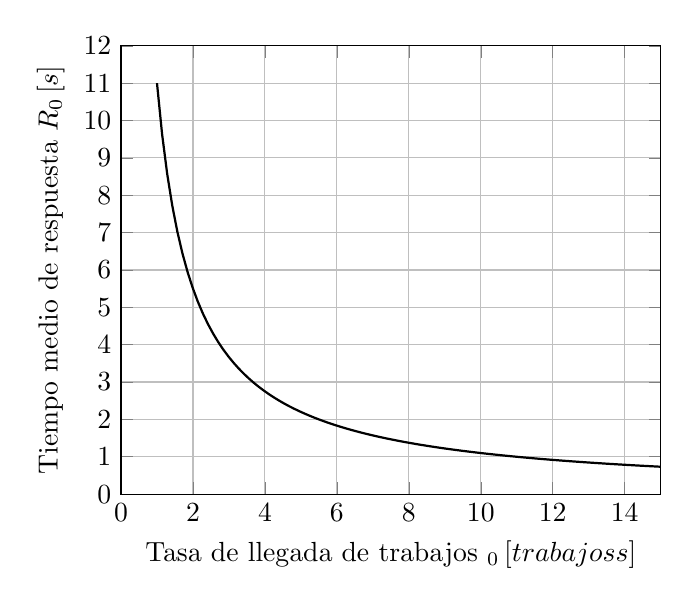
\begin{tikzpicture}
                \begin{axis}[
                    xlabel={Tasa de llegada de trabajos $\lm_0 \left[\unitfrac{trabajos}{s}\right]$},
                    ylabel={Tiempo medio de respuesta $R_0 \left[\unit{s}\right]$},
                    xmin=0, xmax=15,
                    ymin=0, ymax=12,
                    xtick={0,2,...,15},
                    ytick={0,1,...,12},
                    grid=major,
                    legend pos=north west
                ]

                \def\Nt{11} % Número de trabajos
                \addplot[domain=1:15, samples=100, thick] {\Nt/x};
                \end{axis}
            \end{tikzpicture}
            \caption{Límites del Tiempo de Respuesta $R_0$.}
            \label{fig:5.22}
        \end{figure}
        \end{comment}
    \end{enumerate}
\end{ejercicio}
\begin{comment}
\solucion
    \begin{enumerate}
        \item El servidor está cerca del equilibrio porque las demandas son parecidas: $D_1 = 0.09$ y $D_2 = D_3 = 0.08$ segundos/petición.
        \item La carga del servidor es elevada porque el cuello de botella está cerca de la saturación.
        \item El tiempo mínimo de respuesta es 0.25 segundos.
        \item No porque el cuello de botella es el procesador.
        \item El tiempo medio de respuesta es 10.3 segundos.
        \item No porque la disminución de la carga afecta a todo el sistema, no solamente al cuello de botella.
        \item La gráfica muestra una curva creciente con un punto de inflexión en torno a las 8 peticiones por segundo, donde el tiempo medio de respuesta comienza a aumentar rápidamente.
    \end{enumerate}
\end{comment}

\begin{ejercicio}\label{ej:5.23}
    El sistema informático de una empresa, al que se conectan unos 32 clientes de media (suponga un trabajo por cliente), parece que tiene problemas para soportar la carga actual. El administrador ha calculado los siguientes límites optimistas del tiempo de respuesta y de la productividad:
    \begin{align*}
        R_0 &\geq \max\{1.6, 1.1 \times N_T - 4\} \\
        X_0 &\leq \min\left\{\frac{N_T}{5.6}, 0.91\right\}
    \end{align*}
    \begin{enumerate}
        \item El sistema, ¿está realmente soportando una carga elevada?
        
        Para determinar si el sistema está soportando una carga elevada, debemos calcular el punto teórico de saturación (knee point) del sistema. Este se produce cuando:
        \begin{equation*}
            \frac{N_T^*}{5.6} = 0.91
            \Longrightarrow N_T^* = 0.91 \cdot 5.6 \approx 5.096
        \end{equation*}
        Como $N_T = 32 > N_T^* \approx 5.1$, el sistema está soportando una carga elevada.
        \item Haga una estimación del tiempo medio de respuesta del servidor en las condiciones actuales.
        
        Para estimar el tiempo medio de respuesta del servidor, debemos considerar que el sistema está en alta carga. Por tanto, el tiempo mínimo de respuesta del servidor es:
        \begin{equation*}
            R_0^{\text{min}} = 1.1 \cdot N_T - 4 = 1.1 \cdot 32 - 4 = 31.2 \unit{s}
        \end{equation*}
    \end{enumerate}
\end{ejercicio}
\begin{comment}
\solucion
    \begin{enumerate}
        \item La carga es elevada porque el punto teórico de saturación (knee point) está situado en torno a los 5 clientes y en el sistema hay 32 clientes conectados.
        \item El tiempo medio de respuesta del servidor estará situado ligeramente por encima de los 31.2 segundos (parte derecha del límite optimista).
    \end{enumerate}
\end{comment}

\begin{ejercicio}\label{ej:5.24}
    El proceso de modelado de un servidor de base de datos mediante técnicas de análisis operacional ha dado los parámetros que se muestran en la Tabla~\ref{tab:5.24} (los tiempos se expresan en segundos).
    \begin{table}[h]
        \centering
        \begin{tabular}{|c|c|c|}
            \hline
            Dispositivo & $S_i$ & $V_i$ \\
            \hline
            Procesador (1) & $0.15$ & 6 \\
            Disco (2) & $0.05$ & 5 \\
            \hline
        \end{tabular}
        \caption{Parámetros del servidor de base de datos.}
        \label{tab:5.24}
    \end{table}
    El servidor recibe una media de $1.05$ peticiones por segundo. Suponiendo que $R_i = (N_i + 1) \times S_i$, responda a las siguientes cuestiones justificando numéricamente la respuesta.
    \begin{enumerate}
        \item Indique si el servidor está sometido a alta o baja carga.
        
        En este caso no tiene sentido preguntarse por el punto teórico de saturación (knee point) porque estamos ante una red abierta. Calculemos en primer lugar el cuello de botella, y posteriormente su utilización:
        \begin{align*}
            D_1 &= V_1 \cdot S_1 = 6 \cdot 0.15 = \unitfrac[0.9]{s}{peticion} \\
            D_2 &= V_2 \cdot S_2 = 5 \cdot 0.05 = \unitfrac[0.25]{s}{peticion}
        \end{align*}

        El cuello de botella es el procesador porque su demanda de servicio es mayor que la del disco. Por la Ley de la Utilización, tenemos que:
        \begin{equation*}
            U_1 = X_0 \cdot D_1 = 1.05 \cdot 0.9 = 0.945
            \Longrightarrow U_1 = 94.5\%
        \end{equation*}

        Como el cuello de botella tiene una utilización del 94.5\%, el servidor está sometido a alta carga, aunque aún no está saturado.
        \item ¿Cuál es el número medio de trabajos en la cola del procesador?
        
        Por la Ley de Little, el número medio de trabajos en la cola del procesador es:
        \begin{align*}
            Q_1 &= X_1 \cdot W_1
        \end{align*}

        Calculamos en primer lugar $X_1$ empleando para ello la Ley del Flujo Forzado:
        \begin{align*}
            X_1 &= X_0 \cdot V_1 = 1.05 \cdot 6 = 6.3 \unitfrac{trabajos}{s}
        \end{align*}

        A continuación, calculamos el tiempo medio de espera en la cola del procesador:
        \begin{align*}
            W_1 &= R_1 - S_1 = (N_1 + 1) \cdot S_1 - S_1 = N_1 \cdot S_1
        \end{align*}

        Por la Ley de Little, tenemos que:
        \begin{align*}
            N_1 &= X_1 \cdot R_1
            = X_1 \cdot (N_1 + 1) \cdot S_1
            \Longrightarrow N_1 = \dfrac{X_1 \cdot S_1}{1 - X_1 \cdot S_1}
            = 17.181818 \unit{trabajos}
        \end{align*}

        Por tanto, el número medio de trabajos en la cola del procesador es:
        \begin{align*}
            Q_1 &= X_1 \cdot W_1 = 6.3 \cdot 17.181818 \cdot 0.15 = 16.24 \unit{trabajos}
        \end{align*}
        \item Calcule el tiempo medio de respuesta del servidor.
        
        Por la Ley General del Tiempo de Respuesta, el tiempo medio de respuesta del servidor es:
        \begin{align*}
            R_0 &= V_1 \cdot R_1 + V_2 \cdot R_2
        \end{align*}

        Para calcular $R_1$ y $R_2$, necesitamos optener $N_1$ y $N_2$:
        \begin{align*}
            N_i &= X_i \cdot R_i
            = X_i \cdot (N_i + 1) \cdot S_i
            \Longrightarrow N_i = \dfrac{X_i \cdot S_i}{1 - X_i \cdot S_i}
        \end{align*}

        Calculamos ahora $X_1$ y $X_2$ empleando la Ley del Flujo Forzado:
        \begin{align*}
            X_i &= X_0 \cdot V_i
        \end{align*}

        Por tanto:
        \begin{align*}
            N_i &= \dfrac{X_0 \cdot V_i \cdot S_i}{1 - X_0 \cdot V_i \cdot S_i}
        \end{align*}

        Por tanto:
        \begin{align*}
            R_i &= \left(\dfrac{X_0 \cdot V_i \cdot S_i}{1 - X_0 \cdot V_i \cdot S_i} + 1\right) \cdot S_i\\
            R_1 &= 2.72727\unit{s}\\
            R_2 &= 0.0677966\unit{s}
        \end{align*}

        Por tanto, el tiempo medio de respuesta del servidor es:
        \begin{align*}
            R_0 &= V_1 \cdot R_1 + V_2 \cdot R_2 = 16.702619\unit{s}
        \end{align*}
        \item ¿Tendría algún efecto sobre las prestaciones sustituir el procesador por una versión más rápida?
        
        Sí, puesto que el procesador es el cuello de botella del servidor, por lo que la productividad máxima del servidor aumentaría.
        \item Determine cuál sería el cuello de botella del servidor si el procesador y el disco se sustituyen, respectivamente, por versiones 5 y 2 veces más rápidas.
        
        En este caso, la razón de visita no cambia, pero:
        \begin{align*}
            S_1' &= \dfrac{0.15}{5} = 0.03 \\
            S_2' &= \dfrac{0.05}{2} = 0.025
        \end{align*}

        Calculamos la demanda de servicio de cada dispositivo:
        \begin{align*}
            D_1' &= V_1 \cdot S_1' = 6 \cdot 0.03 = \unitfrac[0.18]{s}{peticion} \\
            D_2' &= V_2 \cdot S_2' = 5 \cdot 0.025 = \unitfrac[0.125]{s}{peticion}
        \end{align*}
        En este caso, el cuello de botella seguiría siendo el procesador.
    \end{enumerate}
\end{ejercicio}
\begin{comment}
\solucion
    \begin{enumerate}
        \item La carga es alta porque la tasa de llegadas está cerca de su valor máximo de 1.11 peticiones por segundo.
        \item En la cola del procesador hay una media de 16.24 trabajos.
        \item El tiempo medio de respuesta es de 16.7 segundos.
        \item Sí porque el procesador es el cuello de botella del servidor.
        \item En este caso el cuello de botella seguirá siendo el procesador.
    \end{enumerate}
\end{comment}

\begin{ejercicio}\label{ej:5.25}
    Un sistema interactivo con 3 clientes (suponga un trabajo por cliente) y un tiempo medio de reflexión de 5 segundos se modela mediante los parámetros que se muestran en la Tabla~\ref{tab:5.25} (los tiempos se expresan en segundos):
    \begin{table}[h]
        \centering
        \begin{tabular}{|c|c|c|}
            \hline
            Dispositivo & $S_i$ & $V_i$ \\
            \hline
            Procesador (1) & 0.01 & 15 \\
            Disco (2) & 0.04 & 8 \\
            Disco (3) & 0.08 & 6 \\
            \hline
        \end{tabular}
        \caption{Parámetros del sistema interactivo.}
        \label{tab:5.25}
    \end{table}
    Determine, sabiendo que la productividad del servidor es $\unitfrac[0.49]{trabajos}{s}$, los siguientes valores:
    \begin{enumerate}
        \item El tiempo medio de respuesta del servidor.
        
        Por la Ley del Tiempo de Respuesta Interactivo:
        \begin{align*}
            N_T &= X_0 \cdot (R_0 + Z)
            \Longrightarrow R_0 = \dfrac{N_T}{X_0} - Z = 1.12 \unit{s}
        \end{align*}
        \item Las utilizaciones de cada dispositivo.
        
        Por la Ley de la Utilización, tenemos que:
        \begin{align*}
            U_i &= X_0 \cdot D_i
            = X_0 \cdot V_i \cdot S_i\\
            U_1 &= 0.49 \cdot 15 \cdot 0.01 = 0.0735 = 7.35\% \\
            U_2 &= 0.49 \cdot 8 \cdot 0.04 = 0.1568 = 15.68\% \\
            U_3 &= 0.49 \cdot 6 \cdot 0.08 = 0.2352 = 23.52\%
        \end{align*}
    \end{enumerate}
\end{ejercicio}
\begin{comment}
\solucion
    \begin{enumerate}
        \item $R_0 = 1.1$ s.
        \item $U_1 = 0.07$, $U_2 = 0.16$, $U_3 = 0.24$.
    \end{enumerate}
\end{comment}

\begin{ejercicio}\label{ej:5.26}
    Un servidor web no saturado recibe, por término medio, 4 peticiones de páginas web por segundo. Los tiempos de servicio (expresados en segundos), así como las razones de visita a los dispositivos de este servidor web se indican en la Tabla~\ref{tab:5.26}.
    \begin{table}[h]
        \centering
        \begin{tabular}{|c|c|c|}
            \hline
            Dispositivo & $S_i$ & $V_i$ \\
            \hline
            Procesador (1) & 0.01 & 8 \\
            Disco duro (2) & 0.04 & 4 \\
            Red (3) & 0.03 & 3 \\
            \hline
        \end{tabular}
        \caption{Parámetros del servidor web.}
        \label{tab:5.26}
    \end{table}
    A partir de la información anterior:
    \begin{enumerate}
        \item Calcule la demanda de servicio, la productividad y la utilización de cada dispositivo.
        
        La demanda de servicio de cada dispositivo se calcula como:
        \begin{align*}
            D_i &= V_i \cdot S_i\\
            D_1 &= 8 \cdot 0.01 = \unitfrac[0.08]{s}{peticion} \\
            D_2 &= 4 \cdot 0.04 = \unitfrac[0.16]{s}{peticion} \\
            D_3 &= 3 \cdot 0.03 = \unitfrac[0.09]{s}{peticion}
        \end{align*}

        La productividad de cada dispositivo se calcula por la Ley del Flujo Forzado como:
        \begin{align*}
            X_i &= X_0 \cdot V_i = 4 \cdot V_i\\
            X_1 &= 4 \cdot 8 = 32 \unitfrac{trabajos}{s} \\
            X_2 &= 4 \cdot 4 = 16 \unitfrac{trabajos}{s} \\
            X_3 &= 4 \cdot 3 = 12 \unitfrac{trabajos}{s}
        \end{align*}

        La utilización de cada dispositivo se calcula por la Ley de la Utilización como:
        \begin{align*}
            U_i &= X_i \cdot S_i\\
            U_1 &= 32 \cdot 0.01 = 0.32 = 32\% \\
            U_2 &= 16 \cdot 0.04 = 0.64 = 64\% \\
            U_3 &= 12 \cdot 0.03 = 0.36 = 36\%
        \end{align*}
        
        \item Determine el tiempo mínimo posible de respuesta del servidor web. Justifique la respuesta.
        
        Por la Ley General del Tiempo de Respuesta, el tiempo mínimo de respuesta del servidor web es:
        \begin{align*}
            R_0^{\text{min}} &= \sum_{i=1}^{3} V_i \cdot S_i = \sum_{i=1}^{3} D_i = D_1 + D_2 + D_3\\
            &= 0.08 + 0.16 + 0.09 = \unit[0.33]{s}
        \end{align*}
        \item ¿Qué dispositivo es el cuello de botella del servidor y por qué? ¿Qué valor tendría que tener la tasa de llegadas para que el cuello de botella fuese otro dispositivo? Desde el punto de vista del reparto de la carga entre los componentes del servidor web, ¿estamos ante un sistema equilibrado?
        
        El cuello de botella del servidor es el disco duro, ya que es el dispositivo con mayor demanda de servicio ($D_2 = 0.16\unitfrac{s}{peticion}$). La tasa de llegadas $X_0$ no afecta al dispositivo cuello de botella, ya que este se determina por la demanda de servicio de cada dispositivo. Por último, el sistema no está equilibrado porque la utilización del disco duro es muy superior a la del resto de dispositivos ($U_2 = 64\%$ frente a $U_1 = 32\%$ y $U_3 = 36\%$). 
        \item Calcule la productividad máxima del servidor web. ¿Qué tiempo de servicio debería tener el dispositivo cuello de botella para obtener el doble de esa productividad máxima? Razone la respuesta.
        
        La productividad máxima del servidor web se calcula como:
        \begin{align*}
            X_0^{\text{max}} &= \dfrac{1}{D_b} = \dfrac{1}{D_2} = \dfrac{1}{0.16} = 6.25 \unitfrac{peticiones}{s}
        \end{align*}

        Si quisiéramos obtener el doble de esa productividad máxima, tendríamos que tener:
        \begin{align*}
            X_0^{\text{max}} &= 2 \cdot 6.25 = 12.5 \unitfrac{peticiones}{s} = \dfrac{1}{D_b'}
            \Longrightarrow
            D_b' &= \dfrac{1}{12.5} = 0.08 \unitfrac{s}{peticion}
        \end{align*}

        Por tanto, la demanda de servicio del dispositivo cuello de botella debería ser:
        \begin{align*}
            D_b' = 0.08\unitfrac{s}{peticion}
        \end{align*}

        Por tanto, por un lado necesitaríamos que:
        \begin{align*}
            S_2' &= \dfrac{0.08}{4} = 0.02 \unitfrac{s}{peticion}
        \end{align*}

        No obstante, puesto que $D_3=0.09>D_b'$, también tendríamos que reducir el tiempo de servicio del dispositivo red:
        \begin{align*}
            S_3' &= \dfrac{0.08}{3} = 0.0266667 \unitfrac{s}{peticion}
        \end{align*}
        \item Suponiendo que $R_i=(N_i+1)\cdot S_i$ para cada dispositivo, calcule el tiempo de respuesta del servidor web.
        
        Por la Ley General del Tiempo de Respuesta, el tiempo de respuesta del servidor web es:
        \begin{align*}
            R_0 &= \sum_{i=1}^{3} V_i \cdot R_i
        \end{align*}

        Para calcular $R_i$, necesitamos calcular $N_i$. Por la Ley de Little, tenemos que:
        \begin{align*}
            N_i = X_i \cdot R_i
            = X_i \cdot (N_i + 1) \cdot S_i
            \Longrightarrow N_i &0= \dfrac{X_i \cdot S_i}{1 - X_i \cdot S_i}\\
            N_1 &= \dfrac{32 \cdot 0.01}{1 - 32 \cdot 0.01} = \unitfrac[0.47058]{trabajos}{s} \\
            N_2 &= \dfrac{16 \cdot 0.04}{1 - 16 \cdot 0.04} = \unitfrac[1.7777]{trabajos}{s} \\
            N_3 &= \dfrac{12 \cdot 0.03}{1 - 12 \cdot 0.03} = \unitfrac[0.5625]{trabajos}{s}
        \end{align*}

        Por tanto, el tiempo de respuesta de cada dispositivo es:
        \begin{align*}
            R_i &= (N_i + 1) \cdot S_i\\
            R_1 &= \unit[0.0147]{s} \\
            R_2 &= \unit[0.1111]{s} \\
            R_3 &= \unit[0.0468]{s}
        \end{align*}

        Por tanto, el tiempo de respuesta del servidor web es:
        \begin{align*}
            R_0 &= V_1 \cdot R_1 + V_2 \cdot R_2 + V_3 \cdot R_3 = \unit[0.70271]{s}
        \end{align*}
        \item Calcule el número medio de peticiones en el servidor web. ¿Cómo se llama la ley que ha utilizado?
        
        Por la Ley de Little, el número medio de peticiones en el servidor web es:
        \begin{align*}
            N_0 &= X_0 \cdot R_0 = 4 \cdot 0.70271 = \unit[2.81086]{peticiones}
        \end{align*}
    \end{enumerate}
\end{ejercicio}
\begin{comment}
\solucion
\begin{enumerate}
a) D1=0,08 s/petición al servidor, X1= 32 trabajos/s, U1=0,32; D2=0,16 s/petición al servidor, X2= 16
trabajos/s, U2=0,64; D3=0,09 s/petición al servidor, X3= 12 trabajos/s, U3=0,36;
b) R0min=0,33s. Se produce cuando no hay esperas en la cola de ningún dispositivo por lo que los tiempos 
de respuesta individuales coinciden con los tiempos de servicio.
c) El disco ya que es el que tiene mayor demanda de servicio y, por tanto, mayor utilización. La tasa de
llegadas no influye en cuál es el dispositivo cuello de botella. El sistema no está equilibrado ya que el
disco presenta una utilización muy superior al del resto de dispositivos.
d) X0max=6,25 peticiones/s. Podría pensarse que el tiempo de servicio del disco debería ser la mitad, pero
eso haría que el cuello de botella dejase de ser el disco para pasar a ser la red. Es la red la que entonces
limitaría la productividad máxima y ésta nunca podría superar las 11,1 peticiones/s.
e) R0=0,7 s/petición.
f) N0=2,81 peticiones. Hemos usado la ley de Little.
\end{enumerate}
\end{comment}

\begin{ejercicio}\label{ej:5.27}
    Considere la siguiente parametrización del modelo de un servidor de apuestas deportivas interactivo con 25 clientes en total conectados (suponga un trabajo por cliente) y un tiempo medio de reflexión de 6 segundos (los tiempos de la tabla se expresan en segundos):
    \begin{table}[h]
        \centering
        \begin{tabular}{|c|c|c|}
            \hline
            Dispositivo & $S_i$ & $V_i$ \\
            \hline
            CPU (1) & 0.5 & 4 \\
            Red (2) & 0.75 & 3 \\
            \hline
        \end{tabular}
        \caption{Parámetros del servidor de apuestas deportivas.}
        \label{tab:5.27}
    \end{table}
    A partir de la información anterior:
    \begin{enumerate}
        \item Explique el significado de cada una de las variables que aparecen en las siguientes expresiones y obtenga su valor (no olvide las unidades).
        \begin{align*}
            X_0 &\leq \min\left\{\frac{N_T}{D+Z}, \frac{1}{D_b}\right\}
        \end{align*}
        \begin{itemize}
            \item $X_0$: productividad del servidor, en $\unitfrac{peticiones}{s}$.
            \item $N_T$: número total de clientes conectados al servidor, en unidades. En este caso:
            \begin{align*}
                N_T &= \unit[25]{peticiones}
            \end{align*}

            \item $D$: demanda de servicio del servidor, en $\unitfrac{s}{peticion}$. En este caso:
            \begin{align*}
                D &= D_1 + D_2 = V_1 \cdot S_1 + V_2 \cdot S_2 = 4 \cdot 0.5 + 3 \cdot 0.75 = \unitfrac[4.25]{s}{peticion}
            \end{align*}
            \item $Z$: tiempo medio de reflexión de los clientes, en segundos. En este caso:
            \begin{align*}
                Z &= \unit[6]{s}
            \end{align*}
            \item $D_b$: demanda de servicio del cuello de botella, en $\unitfrac{s}{peticion}$. Esta es la mayor demanda de servicio entre los dispositivos del servidor. En este caso:
            \begin{align*}
                D_b &= \max\{D_1, D_2\} = \max\{V_1 \cdot S_1, V_2 \cdot S_2\} =\\&= \max\{4 \cdot 0.5, 3 \cdot 0.75\} = \max\{2, 2.25\} = \unitfrac[2.25]{s}{peticion}
            \end{align*}
        \end{itemize}
        \item ¿Cuál es el punto teórico de saturación (knee point) del servidor? A la vista de su valor, ¿el sistema se encuentra sometido a baja o alta carga?
        
        El punto teórico de saturación (knee point) del servidor se calcula como:
        \begin{align*}
            \dfrac{N_T^*}{D + Z} = \dfrac{1}{D_b}
            \Longrightarrow N_T^* = \dfrac{D+Z}{D_b} = \dfrac{4.25 + 6}{2.25} \approx \unit[4.555]{clientes}
        \end{align*}
        Como $N_T = 25 > N_T^* \approx 4.555$, el sistema se encuentra sometido a alta carga.
    \end{enumerate}
\end{ejercicio}
\begin{comment}
\solucion
    \begin{enumerate}
        \item $N_T = 25$ clientes; $D = 4.25$ s/petición al servidor (suma de demandas de servicio); $Z = 6$ s (tiempo medio de reflexión de los clientes); $D_b = 2.25$ s/petición al servidor (demanda de servicio del cuello de botella, en nuestro caso: la red). Entonces, $X_0 \leq 0.44$ peticiones al servidor por segundo (productividad del servidor).
        \item El punto teórico de saturación es $N_T^* = 4.6$ clientes. Como $N_T >> N_T^*$ el servidor se encuentra sometido a alta carga. Por lo tanto, $X_0$ será un valor próximo, aunque inferior, a 0.44 peticiones/s.
    \end{enumerate}
\end{comment}

\begin{ejercicio}\label{ej:5.28}
    Un ingeniero informático pretende modelar el servidor de base de datos que está administrando utilizando un modelo basado en redes de colas. Para ello, ha monitorizado el servidor durante 24 horas, contabilizando un total de 15000 peticiones externas al servidor. Durante ese tiempo, el monitor \verb|sar| le ha indicado que el procesador ha estado ocupado un total de 800 minutos y ejecutado 60000 procesos, mientras que se han realizado un total de 135000 accesos al disco duro, habiendo éste trabajado un total de 1200 minutos. Suponiendo que el servidor no está saturado:
    \begin{enumerate}
        \item Calcule la razón de visita, el tiempo de servicio, la productividad y la utilización tanto del procesador como del disco duro.
        
        Los datos proporcionados son:
        \begin{align*}
            X_0 &= \dfrac{15000}{24 \cdot 3600} \approx \unitfrac[0.1736]{peticiones}{s}\\
            U_1 &= \dfrac{800}{24 \cdot 60} \approx 0.5556 = 55.56\%\\
            V_1 &= \dfrac{60000}{15000} = 4 \\
            V_2 &= \dfrac{135000}{15000} = 9 \\
            U_2 &= \dfrac{1200}{24 \cdot 60} = 0.8333 = 83.33\%
        \end{align*}

        Por tanto, tan solo nos falta por calcular el tiempo de servicio y la productividad de cada dispositivo.
        Por la Ley del Flujo Forzado, tenemos que:
        \begin{align*}
            X_i &= X_0 \cdot V_i\\
            X_1 &= 0.1736 \cdot 4 \approx \unitfrac[0.6944]{trabajos}{s} \\
            X_2 &= 0.1736 \cdot 9 \approx \unitfrac[1.5624]{trabajos}{s}
        \end{align*}

        Por la Ley de la Utilización, tenemos que:
        \begin{align*}
            U_i = X_i \cdot S_i
            \Longrightarrow S_i &= \dfrac{U_i}{X_i}\\
            S_1 &\approx \unit[0.800]{s} \\
            S_2 &\approx \unit[0.533]{s}
        \end{align*}
        \item ¿Cuál es la productividad máxima que puede alcanzar este servidor? ¿Y el tiempo de respuesta mínimo?
        
        En primer lugar, calculamos las demandas de servicio de cada dispositivo:
        \begin{align*}
            D_1 &= V_1 \cdot S_1 = 4 \cdot 0.800 = \unitfrac[3.2]{s}{peticion} \\
            D_2 &= V_2 \cdot S_2 = 9 \cdot 0.533 = \unitfrac[4.797]{s}{peticion}
        \end{align*}

        Por tanto, el cuello de botella del servidor es el disco, ya que su demanda de servicio es mayor que la del procesador. Por tanto, la productividad máxima del servidor es:
        \begin{align*}
            X_0^{\max} &= \dfrac{1}{D_b} = \dfrac{1}{D_2} \approx \unitfrac[0.2084]{peticiones}{s}
        \end{align*}

        El tiempo de respuesta mínimo del servidor es:
        \begin{align*}
            R_0^{\min} &= \sum_{i=1}^{2} V_i \cdot S_i = \sum_{i=1}^{2} D_i \approx \unit[7.997]{s}
        \end{align*}
        \item Suponiendo que $W_i = N_i \cdot S_i$, ¿cuál es el tiempo de respuesta actual de los trabajos que llegan al servidor? ¿y el número medio de trabajos en la cola de cada dispositivo?
        
        Por la Ley General del Tiempo de Respuesta, el tiempo de respuesta del servidor es:
        \begin{align*}
            R_0 &= \sum_{i=1}^{2} V_i \cdot R_i
        \end{align*}

        Para calcular $R_i$, necesitamos calcular $N_i$. Por la Ley de Little, tenemos que:
        \begin{align*}
            N_i = X_i \cdot R_i
            = X_i \cdot (W_i+ S_i)
            = X_i \cdot (N_i \cdot S_i + S_i)
            \Longrightarrow N_i = \dfrac{X_i \cdot S_i}{1 - X_i \cdot S_i}
        \end{align*}

        Por tanto, tenemos que:
        \begin{align*}
            N_1 &= \dfrac{X_1 \cdot S_1}{1 - X_1 \cdot S_1} \approx \unit[1.24982]{trabajos} \\
            \\
            N_2 &= \dfrac{X_2 \cdot S_2}{1 - X_2 \cdot S_2} \approx \unit[4.9794021]{trabajos}
        \end{align*}

        Por tanto, el tiempo de respuesta de cada dispositivo es:
        \begin{align*}
            R_i &= W_i + S_i = N_i \cdot S_i + S_i = (N_i + 1) \cdot S_i\\
            R_1 &\approx \unit[1.79985]{s} \\
            R_2 &\approx \unit[3.18702]{s}
        \end{align*}

        Por tanto, el tiempo de respuesta del servidor es:
        \begin{align*}
            R_0 &= V_1 \cdot R_1 + V_2 \cdot R_2 \approx \unit[35.88261]{s}
        \end{align*}

        El número medio de trabajos en la cola de cada dispositivo es:
        \begin{align*}
            Q_i &= X_i \cdot W_i = X_i \cdot N_i \cdot S_i\\
            Q_1 &\approx \unit[0.6943]{trabajos} \\
            Q_2 &\approx \unit[4.1466]{trabajos}
        \end{align*}
    \end{enumerate}
\end{ejercicio}
\begin{comment}
\solucion
    \begin{enumerate}
        \item $V_{cpu} = 4$; $V_{disco} = 9$; $S_{cpu} = 0.8$ s; $S_{disco} = 0.53$ s; $X_{cpu} = 0.69$ trabajos/s; $X_{disco} = 1.56$ trabajos/s; $U_{cpu} = 0.56$; $U_{disco} = 0.83$.
        \item $X_0^{\max} = 0.21$ trabajos/s; $R_0^{\min} = 8.0$ s.
        \item $R_0 = 36$ s; $Q_{cpu} = 0.69$ trabajos; $Q_{disco} = 4.17$ trabajos.
    \end{enumerate}
\end{comment}

\begin{ejercicio}\label{ej:5.29}
    Los parámetros del modelo de un servidor de comercio electrónico (red abierta) son los reflejados en la Tabla~\ref{tab:5.29} (los tiempos de la tabla se expresan en segundos).
    \begin{table}[h]
        \centering
        \begin{tabular}{|c|c|c|}
            \hline
            Dispositivo & $S_i$ & $V_i$ \\
            \hline
            CPU (1) & 0.025 & 8 \\
            HDD (2) & 0.050 & 9 \\
            \hline
        \end{tabular}
        \caption{Parámetros del servidor de comercio electrónico.}
        \label{tab:5.29}
    \end{table}
    La tasa de llegada al servidor es de 1.5 transacciones por segundo.
    \begin{enumerate}
        \item Identifique el cuello de botella y calcule la productividad máxima del servidor.
        
        Calculamos la demanda de servicio de cada dispositivo:
        \begin{align*}
            D_1 &= V_1 \cdot S_1 = 8 \cdot 0.025 = \unitfrac[0.2]{s}{transaccion} \\
            D_2 &= V_2 \cdot S_2 = 9 \cdot 0.050 = \unitfrac[0.45]{s}{transaccion}
        \end{align*}

        El cuello de botella del servidor es el HDD, ya que su demanda de servicio es mayor que la del procesador. Por tanto, la productividad máxima del servidor es:
        \begin{align*}
            X_0^{\max} &= \dfrac{1}{D_b} = \dfrac{1}{D_2} = \dfrac{1}{0.45} \approx \unitfrac[2.22]{transacciones}{s}
        \end{align*}
        \item ¿Cuál es la utilización de la CPU?
        
        Por la Relación Demanda-Utilización, tenemos que:
        \begin{align*}
            U_{cpu} &= X_0 \cdot D_1 = 1.5 \cdot 0.2 = 0.3 = 30\%
        \end{align*}
        \item ¿Cuál sería dicha utilización si la tasa de llegada fuese de $\unitfrac[3]{transacciones}{s}$?
        
        En ese caso el servidor estaría saturado puesto que la tasa de llegada es mayor que la productividad máxima del servidor. La utilización de la CPU máxima que podría alcanzar sería:
        \begin{align*}
            U_{cpu}^{\max} &= X_0^{\max} \cdot D_1 = 2.22 \cdot 0.2 = 0.444 = 44.4\%
        \end{align*}
        \item ¿Cuál sería ahora la productividad máxima del servidor si añadiéramos dos discos duros idénticos al actual suponiendo que la carga se repartiera equitativamente entre los tres discos?
        
        En este caso, la demanda de servicio de cada dispositivo HDD sería:
        \begin{align*}
            D_2' &= S_2\cdot \frac{V_2}{3} = 0.050 \cdot \frac{9}{3} = 0.15 \unitfrac{s}{transaccion}
        \end{align*}

        Por tanto, el cuello de botella del servidor pasaría a ser la CPU, ya que su demanda de servicio es mayor que la del HDD. Por tanto, la productividad máxima del servidor sería:
        \begin{align*}
            X_0^{\max} &= \dfrac{1}{D_1} = \dfrac{1}{0.2} = 5 \unitfrac{transacciones}{s}
        \end{align*}
    \end{enumerate}
\end{ejercicio}
\begin{comment}
\solucion
    \begin{enumerate}
        \item El cuello de botella es el HDD ya que su demanda de servicio ($0.45$ s) es mayor que la de la CPU ($0.2$ s). La productividad máxima del servidor es $X_0^{\max} = 2.22$ transacciones/s.
        \item La utilización de la CPU es $U_{cpu} = 0.3$ (30\%).
        \item En ese caso el servidor estaría saturado. La utilización de la CPU jamás podría ser mayor que el 44\% en este servidor.
        \item Ahora, la productividad máxima del servidor sería $
        \item X_0^{\max} = 5$ transacciones/s (el cuello de botella pasaría a ser la CPU).
    \end{enumerate}
\end{comment}

\begin{ejercicio}\label{ej:5.30}
    Durante las últimas 24 horas, se ha monitorizado un servidor de base de datos no saturado con el fin de obtener un modelo del mismo basado en redes de colas. Como resultado de dicha monitorización, se han obtenido las siguientes medidas:
    \begin{itemize}
        \item Se han contabilizado un total de 54000 consultas al servidor.
        \item La utilización de la unidad SSD es del 60\%.
        \item Cada consulta al servidor requiere una media de 5 accesos a la unidad SSD.
    \end{itemize}
    A partir de la información anterior:
    \begin{enumerate}
        \item Calcule cuánto tiempo, de media, le dedica la unidad SSD a cada consulta que llega al servidor.
        

        Nos piden el valor de $D_i$, puesto que es el tiempo dedicado, de media, a cada petición que llega al \emph{servidor}. Los datos que tenemos son:
        \begin{align*}
            X_0 &= \dfrac{54000}{24 \cdot 3600} \approx \unitfrac[0.625]{consultas}{s}\\
            U_i &= 0.6 \\
            V_i &= 5
        \end{align*}

        Por la Relación Demanda-Utilización, tenemos que:
        \begin{align*}
            U_i = X_0 \cdot D_i
            \Longrightarrow D_i &= \dfrac{U_i}{X_0} = \dfrac{0.6}{0.625} = \unitfrac[0.96]{s}{consulta}
        \end{align*}

        Por tanto, la demanda de servicio de la unidad SSD es $D_{i} = \unitfrac[0.96]{s}{consulta}$.

        
        \item Calcule el tiempo medio de servicio de la unidad SSD.
        
        Por la definición de demanda de servicio, tenemos que:
        \begin{align*}
            D_i &= V_i \cdot S_i
            \Longrightarrow S_i &= \dfrac{D_i}{V_i} = \dfrac{0.96}{5} = \unitfrac[0.192]{s}{consulta}
        \end{align*}
    \end{enumerate}
\end{ejercicio}
\begin{comment}
\solucion
    \begin{enumerate}
        \item La demanda de servicio de la unidad SSD es $D_{ssd} = 0.96$ s (nos piden la demanda de servicio).
        \item El tiempo medio de servicio de la unidad SSD es $S_{ssd} = 0.192$ s.
    \end{enumerate}
\end{comment}

\begin{ejercicio}\label{ej:5.31}
    En una red interactiva formada por un servidor de impresión, durante un tiempo $T = 2$ horas, se encuentran conectados un total de $N_T = 30$ clientes, cada uno imprimiendo un único fichero (1 cliente = 1 fichero). Durante esas dos horas, el tiempo medio entre que un cliente solicita la impresión de un fichero al servidor y éste termina de imprimir dicho fichero (es decir, se completa la tarea) es de $\unit[45]{s}$. Asimismo, el tiempo que transcurre entre que un cliente ve impreso su fichero y vuelve a pedirle al servidor la impresión de otro nuevo es, de media, $\unit[25]{s}$.
    \begin{enumerate}
        \item Calcule la productividad media del servidor.
        
        Como datos, nos proporcionan:
        \begin{align*}
            N_T &= 30 \\
            R_0 &= \unit[45]{s} \\
            Z &= \unit[25]{s}
        \end{align*}

        Por la Ley del Tiempo de Respuesta Interactivo, tenemos que:
        \begin{align*}
            N_T = X_0 \cdot (R_0 + Z)
            \Longrightarrow X_0 &= \dfrac{N_T}{R_0 + Z} = \dfrac{30}{45 + 25} = \dfrac{30}{70} = \unitfrac[0.42857]{transacciones}{s}
        \end{align*}
        \item ¿Cuántos clientes se encuentran, de media, en reflexión?
        
        Por la Ley de Little, el número medio de clientes en reflexión es:
        \begin{align*}
            N_z &= X_0 \cdot Z = 0.42857 \cdot 25 = \unit[10.7143]{clientes}
        \end{align*}
    \end{enumerate}
\end{ejercicio}
\begin{comment}
\solucion
    \begin{enumerate}
        \item La productividad media del servidor es $X_0 = 0.43$ transacciones/s (nos dan $N_T$, $R_0$ y $Z$). El tiempo $T$ no es necesario para calcular la solución.
        \item El número medio de clientes en reflexión es $N_z = 10.7$ clientes.
    \end{enumerate}
\end{comment}

\begin{ejercicio}\label{ej:5.32}
    Suponga que la estación de servicio $i$-ésima de una red de colas que simula el comportamiento de un servidor de base de datos tiene un tiempo de servicio constante igual a 2 s. Suponga que los trabajos (jobs) llegan con la siguiente distribución temporal:
    \begin{itemize}
        \item Durante los primeros 2 segundos no llega ningún trabajo.
        \item En $t = 2$ s llegan 2 trabajos: $J_1$ y $J_2$ (por ese orden).
        \item En $t = 3$ s llega otro trabajo: $J_3$.
    \end{itemize}
    A partir de la información anterior:
    \begin{enumerate}
        \item Calcule los tiempos de espera en la cola y los tiempos de respuesta que experimentan cada uno de los trabajos. Calcule finalmente sus valores medios.
        \item Para el intervalo de medida $[0, 10]$ s, calcule la productividad de la estación de servicio, su utilización y el número medio de trabajos en la cola.
    \end{enumerate}
    % // TODO: Hacer
\end{ejercicio}
\begin{comment}
\solucion
    \begin{enumerate}
        \item Los tiempos de espera en la cola son: $W_i(J_1) = 0$ s, $W_i(J_2) = 2$ s, $W_i(J_3) = 3$ s. El tiempo medio de espera es $W_i = \frac{5}{3} = 1.67$ s. Los tiempos de respuesta son: $R_i(J_1) = 2$ s, $R_i(J_2) = 4$ s, $R_i(J_3) = 5$ s. El tiempo medio de respuesta es $R_i = \frac{11}{3} = 3.67$ s.
        \item La productividad de la estación de servicio es $X_i = 0.3$ trabajos/s, su utilización es $U_i = 0.6$ (60\%) y el número medio de trabajos en la cola es $Q_i = 0.5$ trabajos.
    \end{enumerate}
\end{comment}

\begin{ejercicio}\label{ej:5.33}
    Queremos diseñar un servidor de ayuda a la docencia al que se conectarán unos 30 estudiantes durante las 2 horas que duran las sesiones de prácticas de la asignatura. Este servidor consta de una CPU, un disco duro y una tarjeta de red. Tras la prueba de funcionamiento de 2 horas con 30 estudiantes, se han medido los valores reflejados en la Tabla~\ref{tab:5.33} (los tiempos de la tabla se expresan en segundos):
    \begin{table}[h]
        \centering
        \begin{tabular}{|c|c|c|}
            \hline
            Dispositivo & $S_i$ & $V_i$ \\
            \hline
            CPU (1) & 0.01 & 80 \\
            Disco (2) & 0.5 & 20 \\
            Red (3) & 0.24 & 5 \\
            \hline
        \end{tabular}
        \caption{Parámetros del servidor de ayuda a la docencia.}
        \label{tab:5.33}
    \end{table}
    ¿Cuánto tiempo debería transcurrir, de media, entre que un estudiante recibe la respuesta de este servidor hasta que vuelve a realizar una nueva petición, para que 30 sea precisamente el número ideal de clientes de este servidor?
    % // TODO: Hacer
\end{ejercicio}
\begin{comment}
\solucion
    El tiempo que debería transcurrir, de media, entre que un estudiante recibe la respuesta de este servidor hasta que vuelve a realizar una nueva petición es de 288 s.
\end{comment}
\begin{ejercicio}\label{ej:5.34}
    Partiendo de la hipótesis de que $W_i = N_i \cdot S_i$ para cada estación de servicio de una red de colas que simula el comportamiento de un servidor, demuestre que el cuello de botella del mismo será aquel dispositivo con mayor número medio de trabajos en la cola.\\

    Calculamos el número medio de trabajos en la cola de cada estación de servicio, $Q_i$. Usando la Ley de Little, tenemos que:
    \begin{align*}
        Q_i &= X_i \cdot W_i = X_i \cdot N_i \cdot S_i
    \end{align*}
    Por la Ley de la Utilización, tenemos que:
    \begin{align*}
        U_i &= X_i \cdot S_i
    \end{align*}

    Por tanto, podemos expresar $Q_i$ como:
    \begin{align*}
        Q_i &= U_i\cdot N_i
    \end{align*}

    Calculemos $N_i$:
    \begin{multline*}
        N_i = X_i\cdot R_i = X_i \cdot (W_i + S_i) = X_i \cdot (N_i \cdot S_i + S_i) = X_i \cdot S_i \cdot (N_i + 1)
        \Longrightarrow \\\Longrightarrow N_i = \dfrac{X_i \cdot S_i}{1 - X_i \cdot S_i} = \dfrac{U_i}{1 - U_i}
    \end{multline*}

    Por tanto, podemos expresar $Q_i$ como:
    \begin{align*}
        Q_i &= U_i \cdot \dfrac{U_i}{1 - U_i} = \dfrac{U_i^2}{1 - U_i}
    \end{align*}

    Ahora queremos ver que, efectivamente, si $U_i<U_j$ entonces $Q_i<Q_j$. Para ello, bastará demostrar que la siguiente función es estrictamente creciente:
    \Func{f}{[0,1[}{\bb{R}}{x}{\frac{x^2}{1-x}}

    Calculamos su derivada:
    \begin{align*}
        f'(x) &= \dfrac{(1-x)\cdot 2x +x^2}{(1-x)^2} = \dfrac{2x - 2x^2 + x^2}{(1-x)^2} = \dfrac{2x - x^2}{(1-x)^2} = \dfrac{x(2-x)}{(1-x)^2}
    \end{align*}
    Como $x(2-x) > 0$ para $x \in \left]0, 1\right[$, tenemos que $f'(x) > 0$ para $x \in \left]0, 1\right[$. Por tanto, $f$ es estrictamente creciente en el intervalo $\left]0, 1\right[$, y por tanto si $0 < U_i < U_j < 1$, se cumple que $Q_i < Q_j$. Es decir, la estación de servicio con mayor utilización (es decir, el cuello de botella) también será la que tenga un mayor número de trabajos en la cola.
\end{ejercicio}
\begin{comment}
\solucion
    Si se cumple dicha hipótesis, usando las leyes operacionales se obtiene que: $Q_i = \frac{U_i^2}{1 - U_i}$. Si $0 < U_i < U_j < 1$, se cumple que a) $U_i^2 < U_j^2$ y b) $(1 - U_i) > (1 - U_j)$. Por lo tanto: $\frac{U_i^2}{1 - U_i} < \frac{U_j^2}{1 - U_j}$ (ya que el numerador en el caso de la estación $j$-ésima será mayor y el denominador menor que en el caso de la estación $i$-ésima). Es decir, la estación de servicio con mayor utilización (es decir, el cuello de botella) también será la que tenga un mayor número de trabajos en la cola. Otra forma de razonar esto último consiste en ver que, en el intervalo $[0, 1[$ (que es el rango en el que se van a mover las utilizaciones), $f(x) = \frac{x^2}{1 - x}$ es una función estrictamente creciente.
\end{comment}





\begin{comment}


PROBLEMA 5.32 Suponga que la estación de servicio i-ésima de una red de colas
que simula el comportamiento de un servidor de base de datos tiene un tiempo de
servicio constante igual a 2s. Suponga que los trabajos (jobs) llegan con la siguiente
distribución temporal:
- Durante los primeros 2 segundos no llega ningún trabajo.
- En t=2s llegan 2 trabajos: J1 y J2 (por ese orden).
- En t=3s llega otro trabajo: J3.
a) Calcule los tiempos de espera en la cola y los tiempos de respuesta que
experimentan cada uno de los tres trabajos. Calcule finalmente sus valores
medios.
b) Para el intervalo de medida [0, 10]s, calcule la productividad de la estación de
servicio, su utilización y el número medio de trabajos en la cola.
SOLUCIÓN:
a) Wi(J1) = 0s, Wi(J2) = 2s, Wi(J3) =3s. Valor medio = Wi = 5/3 = 1,67s. Ri(J1) = 2s, Ri(J2) = 4s, Ri(J3)
=5s. Valor medio = Ri= 11/3 = 3,67s.
b) Xi = 0,3tr/s, Ui = 0,6 (60%). Qi = 0,5 trabajos.
PROBLEMA 5.33 Queremos diseñar un servidor de ayuda a la docencia al que se
conectarán unos 30 estudiantes durante las 2 horas que duran las sesiones de
prácticas de la asignatura. Este servidor consta de una CPU, un disco duro y una
tarjeta de red. Tras la prueba de funcionamiento de 2 horas con 30 estudiantes, se han
medido los siguientes valores:
Dispositivo Tiempo de
servicio (s)
Razón de
visita
CPU (1) 0,01 80
DISCO (2) 0,5 20
RED (3) 0,24 5

¿Cuánto tiempo debería transcurrir, de media, entre que un estudiante recibe la
respuesta de este servidor hasta que vuelve a realizar una nueva petición, para que 30
sea precisamente el número ideal de clientes de este servidor?
SOLUCIÓN: 288 s
PROBLEMA 5.34 Partiendo de la hipótesis de que Wi=Ni×Si para cada estación de
servicio de una red de colas que simula el comportamiento de un servidor, demuestre
que el cuello de botella del mismo será aquel dispositivo con mayor número medio de
trabajos en la cola.
SOLUCIÓN:
Si se cumple dicha hipótesis, usando las leyes operacionales se obtiene que: Qi= Ui^2/(1-Ui). Si 0<Ui<Uj<1, se
cumple que a) Ui^2<Uj^2 y b) (1-Ui)>(1-Uj). Por lo tanto: Ui*2/(1-Ui) < Uj^2/(1-Uj) (ya que el numerador en el caso de
la estación j-ésima será mayor y el denominador menor que en el caso de la estación i-ésima). Es decir, la estación
de servicio con mayor utilización (es decir, el cuello de botella) también será la que tenga un mayor número de
trabajos en la cola. Otra forma de razonar esto último consiste en ver que, en el intervalo [0,1[ (que es el rango en el
que se van a mover las utilizaciones), f(x)=x^2/(1-x) es una función estrictamente creciente.
\end{comment}